\documentclass[11pt]{article}
\usepackage[a4paper,margin=18mm]{geometry}
\usepackage[no-math]{fontspec}
\setmainfont{Latin Modern Roman}
\usepackage{amsmath,amssymb,amsthm,xfrac,xspace,hyperref,graphicx,comment}
\excludecomment{DefTralics}
\providecommand{\dpl}{\displaystyle}
\providecommand{\backmatter}{}
\providecommand{\loccit}{\emph{loc. cit.}}

\providecommand{\bibliofont}{\small}
\newcommand{\ie}{i.e.,\xspace}
\newcommand{\eg}{e.g.,\xspace}
\newcommand{\etc}{etc.\xspace}
\newcommand{\cf}{cf.\xspace}
\newcommand{\resp}{resp.\xspace}
\newcommand{\smaller}{\small}
\newcommand{\Subsection}{\subsection}
\newcommand{\Subsubsection}{\subsubsection}
\newcommand{\skpt}{\smallskip}
\emergencystretch=3em

% Begin literal retained input author-preamble.tex
\usepackage[scr=rsfs,cal=euler]{mathalfa}

\newcommand\mto{\mathchoice{\longmapsto}{\mapsto}{\mapsto}{\mapsto}}
\let\epsilon\varepsilon
\newcommand{\cl}{\mathrm{cl}}
\newcommand{\Int}{\mathrm{int}}
\DeclareMathOperator{\id}{id}

\usepackage[capitalize]{cleveref}
\crefdefaultlabelformat{#2\textup{#1}#3}

\crefname{equation}{Equation}{Equations}
\crefname{section}{Section}{Sections}
\crefname{figure}{Figure}{Figures}

\usepackage{graphicx}

\newcommand \cI{{\mathcal I}}
\newcommand \cP{{\mathscr P}}

\newcommand\A{\mathbb A}
\renewcommand\P{\mathbb P}
\newcommand\R{\mathbb R}
\newcommand\T{\mathbb T}
\newcommand\D{\mathbb D}
\newcommand\bS{\mathbb S}
\newcommand\Z{\mathbb Z}

\newcommand\leb{\mathrm{Leb}}

\DeclareMathOperator\diag{diag}
\DeclareMathOperator\Diff{Diff}

\newcommand\qand{\quad \text{and}\quad}

\newtheorem{proposition}{Proposition}[section]
\newtheorem{theorem}[proposition]{Theorem}
\newtheorem{coro}[proposition]{Corollary}
\newtheorem{lemma}[proposition] {Lemma}
\newtheorem{claim}[proposition]{Claim}
\newtheorem{conjecture}[proposition]{Conjecture}

\newtheorem{theo}{Theorem}
\newtheorem{corollary}[theo]{Corollary}
\renewcommand{\thetheo}{\Alph{theo}}

\theoremstyle{definition}
\newtheorem{remark}[proposition]{Remark}
\newtheorem{definition}[proposition] {Definition}
\newtheorem{problem}[proposition]{Problem}
\newtheorem*{remark*}{Remark}


% End literal retained input author-preamble.tex


\makeatletter
\crefname{claim}{Claim}{Claims}
\Crefname{claim}{Claim}{Claims}
\crefname{conjecture}{Conjecture}{Conjectures}
\Crefname{conjecture}{Conjecture}{Conjectures}
\crefname{corollary}{Corollary}{Corollarys}
\Crefname{corollary}{Corollary}{Corollarys}
\crefname{definition}{Definition}{Definitions}
\Crefname{definition}{Definition}{Definitions}
\crefname{lemma}{Lemma}{Lemmas}
\Crefname{lemma}{Lemma}{Lemmas}
\crefname{proposition}{Proposition}{Propositions}
\Crefname{proposition}{Proposition}{Propositions}
\crefname{theorem}{Theorem}{Theorems}
\Crefname{theorem}{Theorem}{Theorems}
\expandafter\def\csname jeplabeltype@main\endcsname{theorem}
\expandafter\def\csname jeplabeltype@HeConj\endcsname{conjecture}
\expandafter\def\csname jeplabeltype@main2sd\endcsname{conjecture}
\expandafter\def\csname jeplabeltype@coroAprime\endcsname{corollary}
\expandafter\def\csname jeplabeltype@coro isotopy\endcsname{corollary}
\expandafter\def\csname jeplabeltype@sheaf\endcsname{proposition}
\expandafter\def\csname jeplabeltype@gluing\endcsname{theorem}
\expandafter\def\csname jeplabeltype@enum:C\endcsname{theorem}
\expandafter\def\csname jeplabeltype@gluing_coro\endcsname{corollary}
\expandafter\def\csname jeplabeltype@gluing2\endcsname{theorem}
\expandafter\def\csname jeplabeltype@def blow-up\endcsname{definition}
\expandafter\def\csname jeplabeltype@prop blow-up\endcsname{proposition}
\expandafter\def\csname jeplabeltype@thm blow-up\endcsname{theorem}
\expandafter\def\csname jeplabeltype@def blow-up2\endcsname{definition}
\expandafter\def\csname jeplabeltype@thm blow-up2\endcsname{theorem}
\expandafter\def\csname jeplabeltype@prop blow-down\endcsname{proposition}
\expandafter\def\csname jeplabeltype@thm blow-down\endcsname{theorem}
\expandafter\def\csname jeplabeltype@actionanglecoordinate\endcsname{lemma}
\expandafter\def\csname jeplabeltype@fonda1\endcsname{claim}
\expandafter\def\csname jeplabeltype@fonda11\endcsname{claim}
\expandafter\def\csname jeplabeltype@fonda12\endcsname{claim}
\expandafter\def\csname jeplabeltype@fonda2\endcsname{claim}
\expandafter\def\csname jeplabeltype@fonda21\endcsname{claim}
\expandafter\def\csname jeplabeltype@fonda22\endcsname{claim}
\expandafter\def\csname jeplabeltype@recap\endcsname{claim}
\expandafter\def\csname jeplabeltype@KPAP\endcsname{proposition}
\expandafter\def\csname jeplabeltype@generalized cap\endcsname{proposition}
\expandafter\def\csname jeplabeltype@fonda3\endcsname{lemma}
\expandafter\def\csname jeplabeltype@Generalized cap\endcsname{lemma}

\expandafter\def\csname jeplabeltype@global\endcsname{figure}
\expandafter\def\csname jeplabeltype@eq psi\endcsname{equation}
\expandafter\def\csname jeplabeltype@eq psi2\endcsname{equation}
\expandafter\def\csname jeplabeltype@eq hat phi\endcsname{equation}
\expandafter\def\csname jeplabeltype@surgery Anosov\endcsname{figure}
\expandafter\def\csname jeplabeltype@eq psi3\endcsname{equation}
\expandafter\def\csname jeplabeltype@def:H\endcsname{equation}
\expandafter\def\csname jeplabeltype@HS\endcsname{equation}
\expandafter\def\csname jeplabeltype@cap surgery\endcsname{figure}
\expandafter\def\csname jeplabeltype@fig:island\endcsname{figure}
\expandafter\def\csname jeplabeltype@fig:oldcoord\endcsname{figure}
\expandafter\def\csname jeplabeltype@cap surgeryS\endcsname{figure}
\AtBeginDocument{\let\jeporiginalLabel\label
\renewcommand{\label}[1]{\ifcsname jeplabeltype@#1\endcsname
\edef\jeplabeltype{\csname jeplabeltype@#1\endcsname}\expandafter\jeporiginalLabel\expandafter[\jeplabeltype]{#1}\else\jeporiginalLabel{#1}\fi}}
\makeatother
\begin{document}
\begin{center}{\Large Stable item 2155}\end{center}
\paragraph{Source and attribution.}
Pierre Berger, \emph{Coexistence of chaotic and elliptic behaviors among analytic, symplectic diffeomorphisms of any surface}, Journal de l’École polytechnique — Mathématiques 10 (2023), publisher version, DOI 10.5802/jep.224. \href{https://jep.centre-mersenne.org/articles/10.5802/jep.224/}{Publisher article}. Authors' text: \href{https://creativecommons.org/licenses/by/4.0/}{CC BY 4.0}.
\paragraph{Editorial problem boundary.}
Prove only TheoremA below: on every closed analytic symplectic surface there exists an analytic symplectomorphism with positive metric entropy and elliptic islands. Retain the exact analytic/symplectic conventions and all new blow-up, involution quotient, Hamiltonian cap, blow-down and genus-wise gluing constructions. Selected existence uses only positive entropy and elliptic definiteness; original ancillary exponent/Hessian descriptions are preserved literally without making their stronger numerical/sign formulations extra claims. Perturbative density, arbitrary isotopy, generalized caps and pseudo-Anosov variants remain surrounding context only.
\paragraph{Difficulty (editorial): H3.}
Analytic bump functions are unavailable, so the desired coexistence cannot be produced by ordinary local smooth pasting. The source constructs an analytic symplectic blow-up, compatible involution quotient and Hamiltonian cap, then blows down the cap boundary while preserving the stochastic piece. It proves the collar gluing and performs the sphere/torus/pants constructions for all genera, remaining substantive surgery obligations after the stated normal-form foundations are allowed.
\paragraph{Editorial transcription note.}
Original author language, mathematics and ordering are preserved. Publisher front matter is replaced by this independent article wrapper. Bibliography is recovered from matching cached publisher HTML, including its TeX formulas. No new proof or mathematical repair is supplied. Surrounding original results are retained for conservative context and are not extra selected corpus claims.
\clearpage

% Begin literal retained input author-body.tex
\begin{theo}[Main result]\label{main}
For every analytic, symplectic and closed surface $(S,\Omega)$, there is an analytic symplectomorphism $f$ of $(S,\Omega)$ such that:
\begin{enumerate}
\item $f$ has positive metric entropy,
\item $f$ displays elliptic islands.
\end{enumerate}
\end{theo}
A symplectic form $\Omega$ on an oriented surface is a nowhere-vanishing volume form. This defines a smooth measure $\leb$ on $S$. A \emph{symplectomorphism} $f$ of $(S, \Omega)$ is a diffeomorphism of $S$ which leaves the volume form $\Omega$ invariant. This is equivalent to say that it is orientation preserving and leaves $\leb$ invariant. Then for $\leb$ a.e.\ point $x\in S$, the limit $\Lambda(x):= \lim_{n\to \infty} \frac1n \log \|D_xf^n\|$ exists. The
\emph{metric entropy} of $f$ is the mean of $\Lambda$. Hence a dynamics has \emph{positive entropy} if it is exponentially sensitive to the initial conditions with positive probability. An \emph{elliptic island} is a domain bounded by a smooth, invariant curve on which the dynamics acts as an irrational rotation. There are many numerical experiments mentioning the coexistence of these two phenomena for symplectic, analytic mappings, however so far no example was proved.

\begin{remark*}
In the proof of \cref{main}, we will show moreover that $S$ minus the support of $\Lambda$ is integrable: the dynamics is equal to the time-one map of a Hamiltonian flow.
\end{remark*}

\section{Introduction}
\subsection{History of the problem}
This problem enjoys a long history. The first exam\-ples of mappings with positive entropy on any surface were discovered by Katok \cite{Ka79}. These examples are isotopic to the identity. Then Katok and Gerber \cite{GK82} obtained mappings with positive entropy on any surface in the isotopy class of any pseudo-Anosov map. Both constructions were smooth but not analytic. In \cite{Ge85}, Gerber constructed real analytic symplectic pseudo-Anosov maps on any surface, which display positive metric entropy but not the coexistence with an elliptic \hbox{island}. In \cite{Pr82}, Przytycki built an example of conservative diffeomorphism of the torus with coexistence of an invariant region with positive entropy and an elliptic island. His construction was infinitely smooth but not analytic. He addressed the problem of whether his construction could be generalized in the analytic class \cite[Rem.\,1, p.\,461]{Pr82}. The issue of this problem was recalled as unclear by Liverani in \cite[Rem.\,2.4, p.\,3]{Li04} where a perturbation of Przytycki's example was studied. Note that \cref{main} solves in particular Przytycki's problem.

In \cite{Go12}, Gorodetski proved that typical examples of analytic symplectic surface maps are such that $\Lambda$ is positive on a set of maximal Hausdorff dimension ($= 2$) and this coexists with elliptic islands. However this leaves open a strong version of the positive entropy conjecture which asserts that ``some typical symplectic dynamics have positive metric entropy'' ($\Lambda$ is positive on a set of positive Lebesgue measure), see \eg \cite[p.\,144]{Si94}. A weaker version of the positive entropy conjecture proposed by Herman \cite{He98} asserts the existence of symplectic mappings $C^\infty$-close to the identity on the disk with positive metric entropy; it implies the density of surface maps with positive metric entropy among those with an elliptic cycle. In \cite{BT19}, the Herman's positive entropy conjecture was proved with Turaev. Our proof used a quotient similar to the examples of Katok and Przytycki. During Katok's memorial conference in 2019, in a conversation with Gorodetski and Kleptsyn, I claimed that the construction of \cite{BT19} should be useful to prove the following analytic counterpart of Herman's positive entropy conjecture \cite{He98} and even the next analytic counterpart of our main result with Turaev.

\begin{conjecture}\label{HeConj}
There exists an analytic and symplectic perturbation of the identity of the closed disk with positive metric entropy.
\end{conjecture}

\begin{conjecture}\label{main2sd}
For every analytic and closed symplectic surface $(S,\Omega)$, for every analytic symplectomorphism $f$ of $S$ displaying an elliptic periodic point, there are analytic and symplectic perturbations of $f$ with positive metric entropy.
\end{conjecture}
These conjectures \ref{HeConj} and \ref{main2sd} might be solved by translating to the analytical setting the strategy\footnote{For an introduction to the proof of \cite{BT19}, one could look at Arnaud's Bourbaki Seminar \cite{Ar19}.} of \cite{BT19}. A first step in this strategy would be to prove the analytic counterpart of Przytycki's example. Following Gorodetski this step was not in reach in a short time, and I bet with him the
existence of such an example in a short time.\footnote{More precisely the bit was that someone would prove within five years the existence of an analytic symplectomorphism of the torus, isotopic to the identity, with positive metric entropy and displaying an elliptic island.} Gorodetski offered me a nice oenological reward, as \cref{coroAprime,coro isotopy} provide many examples concluding our bit:
\begin{corollary}\label{coroAprime}
There exists an analytic and symplectic diffeomorphism $f$ of the closed disk displaying a stochastic island bounded by four heteroclinic bi-links which is robust relative link preservation. \end{corollary}

Let us explain the meaning of the above statement. We recall that a \emph{stochastic island} is a domain $\cI$ on which the maximal Lyapunov exponent $\Lambda$ is positive $\leb$-a.e. A \emph{bi-link} $C$ is a smooth circle equal to the union of two heteroclinic links $C= W^u(P)\cup \{Q\}= W^s(Q)\cup \{P\}$ between saddle fixed points $P$ and $Q$, see \cref{fig:island}.
Note that a symplectomorphism displaying a stochastic island has a positive metric entropy. Given a perturbation of the dynamics, the \emph{bi-link persists} if the union of the stable and unstable manifolds of the fixed points continue to form a differentiable circle. The island is \emph{robust relative link preservation} if for every $C^2$-perturbation such that each of the bi-links persists, the domain bounded by the continuations of these bi-links is still a stochastic island.

We can wonder also what are the isotopy classes of analytic, symplectic surface mappings which display coexistence phenomena. Our techniques enable (at least) to obtain the following:
\begin{corollary}\label{coro isotopy}
Let $(S,\Omega)$ be an analytic and closed symplectic surface and let $C$ be an isotopy class of $\Diff(S)$. If
\begin{itemize}
\item $S$ is the $2$-sphere or the $2$-torus and $C$ is the isotopy class of the identity,
\item or $S$ is a surface of genus $\ge 0$ and $C$ is the isotopy class of a pseudo-Anosov map of $S$,
\end{itemize}
then there is an analytic symplectomorphism $f$ of isotopy class $C$, such that $f$ has positive metric entropy and displays elliptic islands.
\end{corollary}
A natural problem is:
\begin{problem}Realize any isotopy class of surface diffeomorphisms by an analytic and symplectic dynamics displaying coexistence of positive metric entropy and elliptic islands.
\end{problem}
 It seems that the techniques of this work together with the Nielsen-Thurston's classification of symplectic dynamics on surface should lead to a solution of this problem. Another approach would be to prove \cref{main2sd}, which would imply immediately a solution to the latter problem.

The proof of \cref{main} is here completely self contained.

\subsection{Idea and structure of the proof}
All the proofs \cite{Ka79,Pr82,GK82,Li04,BT19} used bump functions to localize the surgery of the dynamics in a subset of the manifold. We recall that there is no analytic bump function. To deal with the analytic case, Gerber \cite{Ge85} showed that the pseudo-Anosov examples of \cite{GK82} persist in a finite co-dimensional submanifold which must intersect the (infinite-dimensional) sub-manifold of analytic maps. However the examples of \cite{Pr82,Li04,BT19}, displaying the sought coexistence, persist actually along an infinite codimensional submanifold: one have to keep intact heteroclinic links. It might be possible to generalize the previous strategy by using an extension of Cartan's Theorem~B. This strategy has been successfully\footnote{Nonetheless, the space of analytic conservative maps is more complicated to deal with than the open cone of analytic Riemannian metric.} applied by Burns-Gerber \cite{burns_gerber_1989} to prove that Donnay's construction \cite{Donnay} of geodesic flow on the $2$-sphere with positive entropy can be performed analytically.

Instead we introduce a new approach:\par\smallskip
\emph{We construct an analytic and symplectic extension of the surface punctured by several saddle points, so that the extended surface remains diffeomorphic to the unpunctured surface, and the analytic continuation of the dynamics on the extended surface displays elliptic islands.}
\par\smallskip
\begin{figure}[htb]
\begin{center}
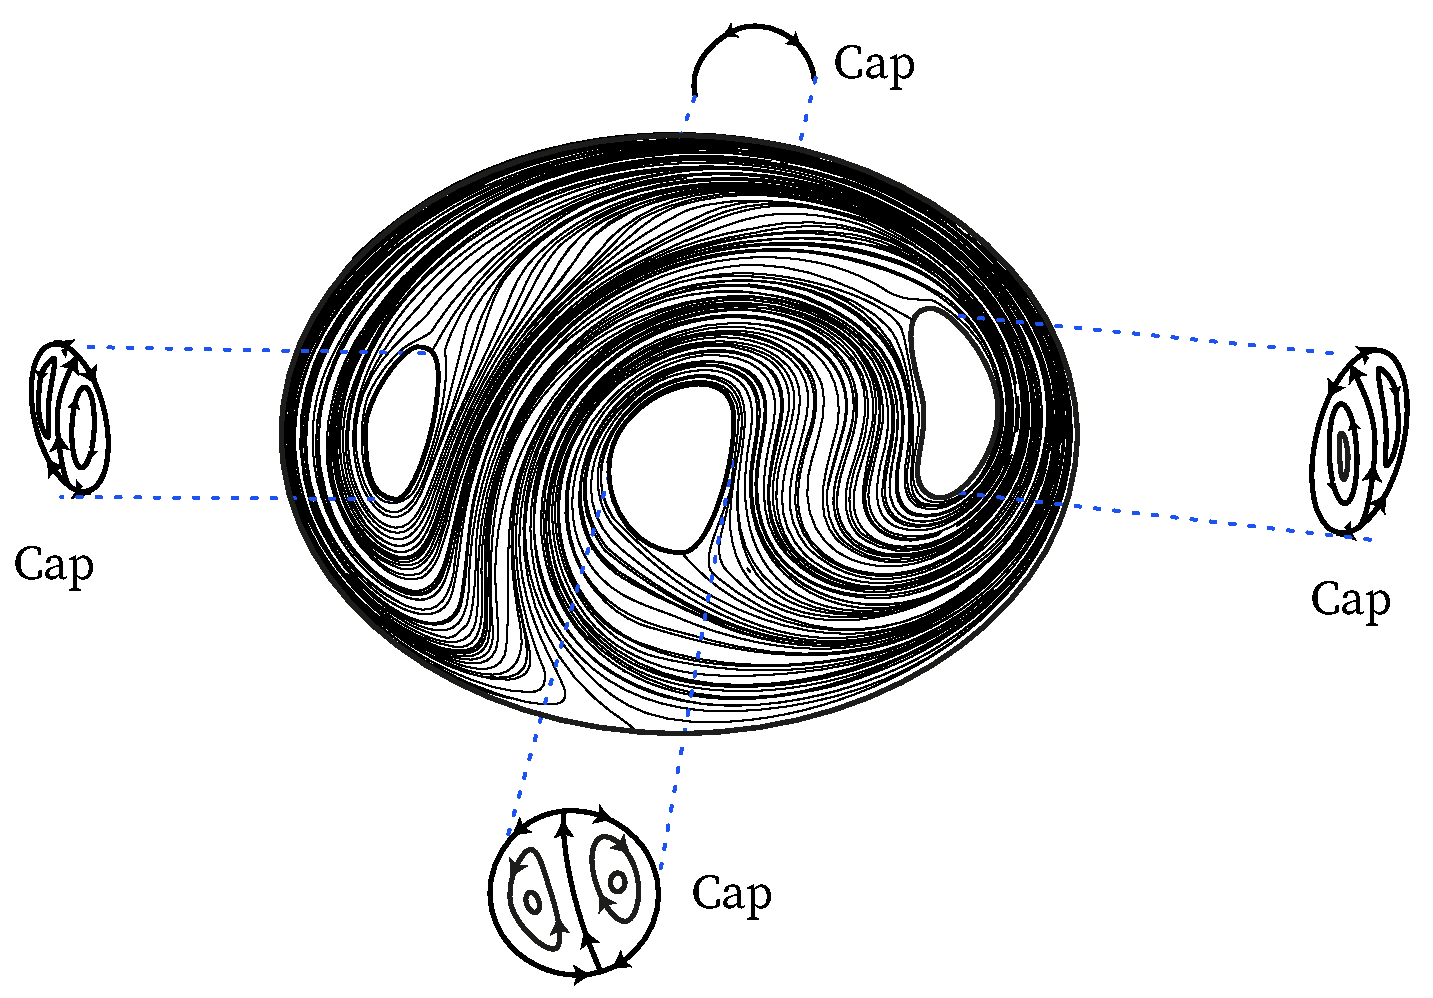
\includegraphics[scale=.38]{../assets/2155/final_surgery_PA.pdf}
\caption{Analytic and conservative dynamics on a sphere displaying coexistence of a stochastic region with elliptic islands.} \label{global}
\end{center}
\end{figure}
We will start with an analytic, conservative dynamics with positive entropy and then we will perform blow-up, quotient, blow-down and connected sums, so that the analytic continuation of
the dynamics is well defined after these operations and displays the sought coexistence properties. There is one ``miracle'' which enables to perform these continuations:

\par\smallskip
\emph{Nearby a saddle point $P$, by Moser's theorem, the dynamics is the time-one map of an analytic Hamiltonian of the form $P+(x,y)\mto H(x\cdot y)$ and such can be analytically lifted to the surface blown up at $P$.}
\par\smallskip\noindent
Indeed, having a flow enables us to perform then analytic surgeries to create an integrable KAM circle which can be in turn be analytically blown down. See \cref{surgery Anosov,cap surgery}.

In \cref{S2}, we present a general framework to perform these surgeries, the main novelties~in these operations lie in providing sufficient conditions to obtain the analytic and symplectic continuation of a dynamic after surgery. First we recall the definition of analytic and symplectic manifolds and their mappings in \cref{S21}. Then, in~\cref{S22}, we state \cref{gluing} which is a general theorem used in the proof of all the surgery's results of Section \ref{S2}. In \cref{S23}, we present \cref{gluing2} which enables to glue two analytic and symplectic surface dynamics. In \cref{S24}, we introduce \cref{thm blow-up,thm blow-up2} which allow to blow up at a hyperbolic periodic orbit of an analytic surface symplectomorphism. Finally in \cref{S25}, we present \cref{thm blow-down} which enables to blow-down a nearby integrable circle of an analytic and symplectic surface dynamics. This last operation was perhaps the most unexpected by dynamical experts.

In Section \ref{S3}, we use the surgery theorem of the previous section to construct the stochastic sphere with four holes and the integrable caps depicted in \cref{global}. We~start in \cref{S31} with a linear Anosov map on the $2$-torus, then we blow-up four of its fixed points à la Przytycki to define an analytic symplectic diffeomorphism of the $2$-torus $\hat \T^2$ without four disks, then we quotient it à la Katok to define an analytic symplectic diffeomorphism of the $2$-sphere $\hat \bS$ without four disks in \cref{S32}. These steps were already performed in \cite{BT19} and are depicted in \cref{surgery Anosov}. This is the construction of the stochastic spheres with four holes. Importantly nearby each component of the boundary, the dynamics is the time-one map of a Hamiltonian $H$ on a semi-closed annulus.

Then we propose a new construction to obtain the integrable caps. In \cref{S33}, we consider an analytic extension of $H$ to a symmetric semi-closed annulus $\A_\Delta (\epsilon)$. Then we perform surgeries as depicted in \cref{cap surgery}. First we define a neighborhood~$\tilde \Delta$ of the circle $\partial \A_\Delta (\epsilon)$ such that $\tilde \Delta$ has five sides, among which $\partial \A_\Delta (\epsilon)$ and two segments of orbits. We glue the two remaining sides to obtain a closed disk $\widehat \Delta$ with two holes endowed with an analytic Hamiltonian. The borders of both holes are orbits of the systems. Thus Theorem 2.14 enables to blow-down them to obtain a closed disk $\Delta$ endowed with an analytic Hamiltonian. The time-one map of this Hamiltonian is the integrable cap. Eventually, in \cref{S34}, we show that the integrable cap recaps analytically any holes of the stochastic sphere with holes.

This allows in \cref{S4} to prove the main theorem and the corollaries of its proof. In \cref{S41}, we start by proving \cref{main} when the surface is a sphere; the construction is depicted by \cref{global}. Following the number of recaped holes, coexistence phenomena are obtained on a disk (which contains the stochastic island of \cref{coroAprime}), a cylinder or a pair of pants. The boundary of these can be glued together to form any closed symplectic surface, and so obtain \cref{main}. A careful study enables to obtain an analytic, symplectic diffeomorphism of the torus isotopic to the identity, as wondered by Gorodetski and part of \cref{coro isotopy}.

In \cref{S42}, we prove the remaining part of \cref{coro isotopy} regarding surface mappings isotopic to a pseudo-Anosov map. We will start with the example of analytic pseudo-Anosov map of \cite{Ge85}, which can represent any isotopy class of orientation preserving pseudo-Anosov maps (see also \cite{GK82}). From this, \cref{thm blow-up2} enables to blow-up one of its hyperbolic periodic orbit, and obtain an analytic and symplectic dynamics on the surface which is integrable nearby the holes. Then we proceed as in \cref{S33}-\ref{S34} to recap these holes. The only difference is that the normal form \cite{Mo56} at the saddle points is more general and that we will be working on a $2$-lifting of the previous construction. Caps will be replaced by a certain \emph{generalized cap} given by \cref{generalized cap,Generalized cap}. The proof of the lemma follows the same lines as \cref{S33}.\enlargethispage{.5\baselineskip}%

\subsubsection*{Acknowledgements}
I am grateful to A.\,Gorodetski and V.\,Kleptsyn for their encouragements. I am thankful to R.\,Krikorian and P.~Le Calvez for nice conversations. I am very grateful to S.\,Biebler for his careful reading.

\section{Dynamical analytic and symplectic surgeries}\label{S2}

In this section we revisit different surgery techniques which enable to construct a new symplectic and analytic surface from an existing one. The main novelty of this section will be to extend these operations to some symplectic and analytic \emph{dynamics} on these surfaces (see \cref{gluing2,thm blow-up,thm blow-down}). These will be the basic ingredients of the proof of the main theorems; hopefully these will be also useful for other problems.

\subsection{General definitions}\label{S21}
To perform analytical surgeries on surfaces, we shall work with their manifold structure (rather than working on them as embedded into~$\R^3$).

We recall that an analytic manifold (\resp with boundary or with corner) $M$ of dimension $n$ is a paracompact space \emph{modeled} on $\R^n$ (\resp $\R_+\times \R^{n-1}$ or $\R_+^n$). By~\emph{modeled} we mean that there is an atlas of $M$ formed by charts $\phi_i: U_i\subset M\to V_i\subset \R^n$ (\resp $\R_+\times \R^{n-1}$ or $\R_+^n$) for an open covering $(U_i)_{i\in I}$ of $M$ so that the coordinate changes $\phi_j\circ \phi^{-1}_i$ are analytic diffeomorphisms on their definition domains (which are open subsets of \resp $\R^n$, $\R_+\times \R^{n-1}$ or $\R_+^n$). An \emph{analytic (or $C^\omega$) structure} is a maximal atlas. Note that the differentials of these charts form an analytic atlas (and so a $C^\omega$-structure) on the tangent space $TM$ of $M$. A \emph{map $f: M\to N$ between two analytic manifolds is analytic (or of class $C^\omega$)} if there are $C^\omega$-atlases $(\phi_i)_{I}$ and $(\psi_j)_{J}$ of $M$ and $N$ such that $\phi_i\circ f\circ \psi^{-1}_j$ is analytic on its definition domain for every $i\in I$ and $j\in J$. Then this property is satisfied with any greater $C^\omega$-atlas of $M$ and $N$ and in particular with the $C^\omega$-structures.

An analytic symplectic form $\Omega:TM^{\otimes 2}\to \R$ on $M$ is an analytic, bilinear, closed and non-degenerate form. Then we say that $(M,\Omega)$ is an \emph{analytic symplectic manifold}.
An analytic map $f$ between two symplectic manifolds $(M,\Omega)$ and $(N,\Omega')$ is \emph{symplectic} if it pushes forward $\Omega$ to $\Omega'$: $f^*\Omega = \Omega'$. Then we say that $f$ is of class $C^\omega_\Omega$. If $(M,\Omega)=(N, \Omega')$ and if $f$ is a diffeomorphism, then $f$ is an analytic \emph{symplectomorphism} of $(M,\Omega)$. The space of analytic symplectomorphisms of $(M,\Omega)$ is denoted by $\Diff^\omega_\Omega(M)$.

A manifold is \emph{closed} when $M$ is compact and boundary less.
When $M$ is a surface with boundary or corner, we recall that it is modeled on $\R_+\times \R$ or $\R_+^2$ via an atlas $(\phi_i)_i$.
The boundary $\partial M$ of $M$ is
\[
\bigcup_i \phi^{-1}_i(\{0\}\times \R)\quad\text{or respectively}\quad \bigcup_i \phi^{-1}_i(\{0\}\times \R\cup \R\times \{0\}),
\]
while the corner of $M$ is $\bigcup_i \phi^{-1}_i(\{0\})$.
\begin{remark}
Given a submanifold $N \subset M$, we will denote $\partial N$ the boundary of $N$ as manifold and not the subset $\cl(N) \setminus \Int(N)$. These are different in general.
\end{remark}



The above (classical) definitions may sound over formal, however they will turn out to be very efficient to verify the analyticity of the dynamics lifted by the surgeries. Also this formalism clarifies that being analytic for a mapping is a local property:

\begin{proposition}\label{sheaf}
A map $f: M\to N$ between two analytic manifolds $M$ and $N$ is analytic iff
there exists an open covering $(V_i)_{i\in I}$ of $M$ such that each restriction $f|V_i$ is analytic.
Moreover if $f: M\to N$ is analytic, then its restriction to any open subset of $M$ is analytic.
\end{proposition}
In more sophisticated terms, the latter implies that the space of analytic maps defines a sheaf.

\subsection{A general result for analytic and symplectic surgeries}\label{S22}
Let $M$ be a $C^\omega$-manifold possibly with boundaries and possibly not connected. Let $O$ be an open subset of $M$ and let $J\in \Diff^\omega(O)$ be an \emph{analytic involution}: $J^2=\id$.
Note that $J$ must preserve the boundary of $M$: $J(O \cap \partial M)= J(O)\cap \partial M$. Let $M/J$ be the quotient of $M$ by the equivalence relation defined by $x\sim x'$ if either $x=x'$, or $x\in O $ and $x'= J(x)$.
Denote $\pi: M\to M/J$ the canonical projection.
The following will be the basis of all the surgeries performed:

\begin{theorem}\label{gluing} Assume $J$ without fixed point and satisfying the following separation criterion:
\begin{enumerate}\renewcommand{\theenumi}{C}
\item\label{enum:C}
There is a neighborhood $W $ of $\cl(O)\setminus O $ in $M$ such that $J(W\cap O)$ and $W \cap O $ are disjoint.
\end{enumerate}
Then there exists a unique $C^\omega$-manifold structure on $M/J$ such that $\pi: M\to M/J$ is an analytic local diffeomorphism. Also for every analytic manifold $M'$, a map $f: M/J \to M'$ is analytic iff $f\circ \pi $ is analytic.
\end{theorem}

\begin{proof} It suffices to show that the following set is a closed analytic submanifold of $M\times M$:
\[E:=\{(x,y)\in M\times M: x=y\text{ or } y=J(x)\text{ with } x\in O\}\]
such that $pr_1: E\to M$ is a local diffeomorphism. Indeed \cite[\textsection 5.9.5]{Bo67} implies then the theorem.

Note that $\mathrm{Diag}:=\{(x,x): x\in M\}$ and $\mathrm{Graph}(J)=\{(x,J(x)): x\in O\}$ are submanifolds. Furthermore, they are disjoint since $J$ does not fix any points. Furthermore, $\mathrm{Diag}$ is obviously closed and we can show that
$\mathrm{Graph}(J)$ is closed. If $(x_n,J(x_n))_n$ converges to some $(x,y)\in M^2$ which is not in $\mathrm{Graph}(J)$, then $x$ is in $\cl(O)\setminus O$ and so in $W$. Thus $x_n\in W$ for every $n$ large. Therefore $J(x_n)$ is not in $W$ by \eqref{enum:C}. So $y$ belongs to the closed set
$O\setminus \Int(W)$. Using that $J$ is an involution, it comes that $x\in J(O\setminus \text{int}\, W)\subset O$. A contradiction. This shows that $E$ is a disjoint union of two closed $C^\omega$-submanifolds of $M\times M$ and so is a closed $C^\omega$-submanifold of $M\times M$. Also $pr_1: E\to M$ is clearly a local diffeomorphism.
\end{proof}

The latter proposition enables to preserve the symplectic structure:
\begin{coro}\label{gluing_coro}
Under the assumptions of \cref{gluing}, if $\Omega$ is an analytic symplectic form on $M$ such that $\Omega|O $ is left invariant by $J$, then there is a canonical analytic symplectic form on $M/J$ for which $\pi$ is symplectic.
\end{coro}
\begin{proof}
We recall that $\Omega$ is a mapping from $TM^{\otimes 2}$ to $\R$. Note that $DJ$ acts on $TM^{\otimes 2}|O$ as $(x,u,v)\mto (J(x), D_xJ(u), D_xJ(v))$; it is an involution without fixed point satisfying condition \eqref{enum:C}. Thus by the latter proposition $TM^{\otimes 2}/DJ$ is an analytic manifold. By uniqueness
$TM^{\otimes 2}/DJ$ is equal to $T(M/J)^{\otimes 2}$. As $J$ leaves $\Omega$ invariant,
by the last statement of \cref{gluing},
it is pushed forward by the projection
$TM^{\otimes 2}\to TM^{\otimes 2}/DJ= T(M/J)^{\otimes 2}$ to an analytic symplectic form on $M/J$.
\end{proof}

\Subsection{Symplectic gluing and induced dynamics}\label{S23}
\begin{theorem}\label{gluing2}
Let $(M_1,\Omega)$ and $(M_2,\Omega)$ be two analytic symplectic surfaces with boundary. For $1\le i\le 2$, let
$C_i$ be a component of $\partial M_i$, let $V_i\subset M_i$ be a neighborhood of $C_i$ in $M_i$
and let $f_i\in \Diff^\omega_\Omega(M_i)$ which leaves $C_i$ invariant: $f_i(C_i) = C_i$.
Assume that there exist $\eta>0$ and a map $\Phi: V_1\sqcup V_2\to \R/\Z\times (-\eta,\eta)$ such that:
\begin{enumerate}
\item the restriction of $\Phi$ to $V_1$ is a $C^\omega$-symplectomorphism onto
$\R/\Z\times (-\eta, 0]$ and the restriction of $\Phi$ to $V_2$ is a $C^\omega$-symplectomorphism onto $\R/\Z\times [0, \eta)$,
\item there is an analytic symplectomorphism $f_{1,2}$ from a neighborhood of $\R/\Z\times \{0\}$ into $\R/\Z\times \R$ such that for each $i\in \{1,2\}$, $f_{1,2}\circ \Phi|V_i$ coincides with $ \Phi\circ f_i $ nearby $C_i$.
\end{enumerate}
Then the gluing of $M_1$ and $M_2$ at $C_1$ and $C_2$ by $(\Phi|C_2)^{-1}\circ \Phi|C_1$ supports a structure of analytic and symplectic manifold $(M,\Omega)$ so that there exists $f\in \Diff^\omega_\Omega(M)$ satisfying $f|M_i=f_i$.
\end{theorem}
\begin{proof} We are going to apply \cref{gluing} with the symplectic manifold:
\[M:= (M_1\setminus C_1)\sqcup (M_2\setminus C_2)\sqcup \R/\Z\times(-\eta, \eta),\]
its open subset:
\[O:= (V_1\setminus C_1)\sqcup (V_2\setminus C_2)\sqcup \R/\Z\times \{r\in (-\eta, \eta): r\neq 0\} \]
and the $C^\omega_\Omega$-involution $J$ defined by:
\[J:= x\in O\mto
\begin{cases}
\Phi(x) & \text{if } x\in V_1\sqcup V_2,\\
\Phi^{-1}(x) & \text{otherwise}.\\
\end{cases}
\]
Note that Condition \eqref{enum:C} of \cref{gluing} is satisfied with:
\[W:=
\left(M_1\sqcup M_2\setminus \Phi^{-1}(\R/\Z\times (-\eta/2,\eta/2))\right)\sqcup
\R/\Z\times (-\eta/2,\eta/2).\]
Hence there is a unique $C^\omega_\Omega$-structure on $ M/J$ such that $\pi: M\to M/J$ is of class $C^\omega_\Omega$.
Note that for $\eta'<\eta$, there are canonical inclusions
$(M_1\setminus C_1)\sqcup (M_2\setminus C_2)\hookrightarrow M/J$ and $\R/\Z\times (-\eta', \eta')\hookrightarrow M/J$ and their images form a open covering of $M/J$ on which the maps $\pi\circ f_1$, $\pi\circ f_2$ and $\pi\circ f_{12}$ agree. So, by \cref{sheaf}, these maps define a $C^\omega_\Omega$\nobreakdash-map~$f$ of $M/J$. As $\pi$ is a local diffeomorphism, $f$ is a local diffeomorphism. We~conclude by noting that $f$ is a homeomorphism as it is the gluing of two homeomorphisms.
\end{proof}
\begin{remark} In \cref{gluing2}, we can assume that $M_1=M_2$ provided that $C_1\neq C_2$.
\end{remark}
\subsection{Symplectic blow-up and induced dynamics}\label{S24}
Let $(M,\Omega)$ be a symplectic $C^\omega$\nobreakdash-sur\-face.
A blow-up at a point $P\in M\setminus \partial M$
consists of replacing $P$ by a circle and a neighborhood $V$ of $P$ by symplectic polar coordinates. Usually these coordinates are parametrized by a Möbius strip, here we will parametrize them by a semi-closed annulus:
\[\A(\delta):= \R/2\pi \Z \times [0, \tfrac12 \delta^2), \quad \text{ for } \delta>0.\]

We will blow-up $P$ to the circle $ \R/2\pi \Z \times \{0\}=\partial \A(\delta)$ which is the boundary of $\A(\delta)$. We will obtain an analytic symplectic surface $\hat M$ with an extra hole surrounded by the circle replacing $P$.
This surgery will be used in \cref{S31,S42}, and an example of such is depicted \cref{surgery Anosov} [left-center].
Let us precise the construction of such a blow-up. We endow the following with the standard symplectic form $dx\wedge dy$ or $d\theta\wedge dr$:
\begin{gather*}
\D(\delta)=\{(x,y)\in \R^2: x^2+y^2< \delta^2\},\\
\A(\delta)= \R/2\pi \Z \times [0, \tfrac12 \delta^2)\qand
\mathring \A(\delta)= \R/2\pi \Z \times (0, \tfrac12 \delta^2),\end{gather*}
The blow-up depends on the choice of a $C^\omega_\Omega$-chart $\varphi$ of a neighborhood $V$ of $P$ of the form:
\[\varphi: \D(\delta)\to V \subset M \qand \varphi(0)=P.\]

We glue the surfaces $\A(\delta)$ and
$M\setminus \{P\}$ at the open subsets $\mathring\A(\delta) $ and $V \setminus \{P\}$ with
the symplectomorphism:
\begin{equation} \label{eq psi}\psi: (\theta,r)\in\mathring\A(\delta) \mto \varphi\bigl(\sqrt{2r } \cdot \cos (\theta), \sqrt{2r }\cdot \sin (\theta)\bigr)\in V \setminus \{P\}.\end{equation}
To apply \cref{gluing}, we define the involution $J$ of $O:=\mathring\A(\delta)\sqcup
V \setminus \{P\}$ which coincides with $\psi$ on $\mathring\A(\delta)$ and with $\psi^{-1}$ on $V \setminus \{P\}$.

\begin{definition}\label{def blow-up}
The quotient $ \hat M:=\mathring\A(\delta) \sqcup (M\setminus \{P\}) /J$ endowed with the canonical projection $p:\hat M\to M$ is a \emph{blow-up} of $M$ at $P$ given by $\varphi$. \end{definition}
Note that $J$ has no fixed point. Also Condition \eqref{enum:C} of \cref{gluing} is satisfied
with $W= \A(\delta/3)\sqcup M\setminus \psi (\A(2\delta/3))$. By \cref{gluing_coro}, it comes:
\begin{proposition}\label{prop blow-up} The space $\hat M$ has a
canonical structure of analytic and symplectic surface.
\end{proposition}

Here is the first key ingredient of the proof of the main theorem.
\begin{theorem}\label{thm blow-up}
Let $f\in \Diff^\omega_\Omega(M)$ which displays a hyperbolic fixed point $P$ with positive eigenvalues.
Then there is a blow-up $p: (\hat M, \Omega)\to (M,\Omega)$ of $M$ at $P$ and a~lifting $\hat f\in \Diff^\omega_\Omega(\hat M)$:
\[p\circ \hat f= f\circ p.\]
Moreover, there are coordinates $\hat \psi: \A(\delta) \to \hat V$ of a neighborhood $\hat V$ of $p^{-1}(P)$,
a function $\Lambda\in C^\omega([0,\tfrac12 \delta^2),\R)$ with positive derivative and a Hamiltonian $H\in C^\omega (\A(\delta), \R)$ whose time-one map $\phi_H^1$ satisfies:
\[\hat f \circ \hat \psi(\theta, r) = \hat \psi\circ \phi_H^1(\theta,r) \qand H (r,\theta)= \Lambda (r \cdot \sin(2\theta)),\]
for every $(\theta,r)$ nearby $\R/2\pi \Z\times \{0\}$.

\end{theorem}
\begin{proof}
By \cite{Mo56}, there exist $\delta>0$, a $C^\omega_\Omega$-chart $\varphi: \D(\delta)\to V$ of a neighborhood~$V$ of~$P\in M$ and an analytic and positive function $\lambda: \D(\delta)\to \R $ such that every $(x,y)$ small satisfies:
\[\varphi^{-1}\circ f\circ \varphi (x,y)= (\exp(\lambda(x\cdot y)) \cdot x, \exp(-\lambda(x\cdot y))\cdot y).\]
We perform the blow-up using this map $\varphi$.
Let $p: \hat M \to M$ be the blow-up obtained. Let $\psi: \mathring \A(\delta)\to V\setminus \{P\}$ be given by \cref{eq psi}.
Let $\hat \psi: \mathring \A(\delta)\to \hat M$ be the lifting of $\psi$: it satisfies $p\circ \hat \psi= \psi$.

Let $\Lambda$ be an integral of the function $\lambda$ so that $\Lambda(0)=0$. Note that $D\Lambda>0$ and that $\varphi^{-1}\circ f\circ \varphi $ coincides with the time-one of the flow of the Hamiltonian $(x,y)\mto \Lambda (x\cdot y)$. Hence the time-one map $\phi_H^1$ of the flow of the Hamiltonian
\[H: (\theta, r)\in \A (\delta) \mto \Lambda(r\cdot \sin(2\theta))\]
coincides with $\psi^{-1}\circ f\circ \psi$ on the intersection of their definition domains. Thus by
\cref{gluing}, the maps $f|M\setminus \{P\}$ and
$\phi^1_H$ define a map $\hat f\in \Diff^\omega_\Omega(\hat M)$ which satisfies the sought properties.
\end{proof}
Actually, in the proof of the main theorem, we will blow-up the surface at a finite set $\cP\subset M$.
The blow-up of $M$ at $\cP$ depends on the choice of a $C^\omega_\Omega$-chart
$\varphi$ of a neighborhood $V$ of $\cP$ and of the form:
\[\varphi: \D(\delta)\times \cP \to V\subset M\qand \varphi(\{0\}\times \cP)=\cP.\]
We glue the surfaces
$ \A(\delta)\times \cP$ and
$ M\setminus \cP$ at the open subsets $ \mathring\A(\delta)\times \cP $ and $V \setminus \cP$ with
the symplectomorphism:
\begin{equation} \label{eq psi2}\psi: (\theta,r,P)\in\mathring\A(\delta) \times \cP \mto \varphi\bigl(\sqrt{2r } \cdot \cos (\theta), \sqrt{2r }\cdot \sin (\theta),P\bigr)\in V \setminus \cP.\end{equation}
We apply \cref{gluing_coro}, with the involution $J$ of $O=\mathring\A(\delta)\times \cP\sqcup
V \setminus \cP$ which coincides with $\psi$ on $\mathring\A(\delta)\times \cP$ and with $\psi^{-1}$ on $V \setminus \cP$, to obtain similarly:
\begin{definition}\label{def blow-up2} The quotient $\hat M:= M/ J$ endowed with the canonical projection $p:
\hat M\to M$ is a \emph{blow-up} of $M$ at $\cP$ given by $\varphi$. The space $\hat M$ has a unique analytic and symplectic surface structure such that $p$ is analytic. \end{definition}
A similar proof to the one of \cref{thm blow-up} gives:
\begin{theorem}\label{thm blow-up2}
Let $f\in \Diff^\omega_\Omega(M)$ which displays a finite union of hyperbolic periodic orbits $\cP$ with positive eigenvalues.
Then there is a blow-up $p: (\hat M, \Omega)\to (M,\Omega)$ at $\cP$ and a lifting $\hat f\in \Diff^\omega_\Omega(\hat M)$:
\[p\circ \hat f= f\circ p.\]
Moreover, there are coordinates $\hat \psi: \A(\delta)\times \cP \to \hat V$ of a neighborhood $\hat V$ of $p^{-1}(\cP)$ and a Hamiltonian $H\in C^\omega (\A(\delta)\times \cP, \R)$ whose time-one map $\phi_H^1$ satisfies:
\[\hat f \circ \hat \psi (\theta, r,P) = \hat \psi(\phi_H^1(\theta,r,P), f(P))\text{ and } H (r,\theta,P)= \Lambda (r \cdot \sin(2\theta),P)= H(r,\theta, f(P)) \]
for every $(\theta,r,P)$ nearby $\R/2\pi \Z\times \{0\}\times \cP$
and for a function $\Lambda\in C^\omega([0,\tfrac12 \delta^2) \times \cP,\R)$ with positive first derivative.
\end{theorem}
\subsection{Symplectic blow-down}\label{S25}
The symplectic blow-down is the inverse operation of the blow-up. This surgery will be used in \cref{S33,S42} as depicted by \cref{cap surgery,cap surgeryS} [center-right].

Let $(\hat M,\Omega)$ be a symplectic surface with boundary $\partial \hat M$. Assume that a component of $\partial \hat M$ is a circle $C$. Let:
\[\hat \psi: \A(\delta)=\R/2\pi \Z \times [0, \tfrac12 \delta^2)\to \hat U\]
be a $C^\omega$-symplectomorphism onto a neighborhood $\hat U$ of $C$ in $\hat M$. Put:
\begin{equation} \label{eq hat phi} \hat \varphi:\bigl(\sqrt{2r } \cdot \cos (\theta), \sqrt{2r }\cdot \sin (\theta)\bigr)\in \D(\delta)\setminus \{0\} \mto \hat \psi(\theta,r)\in \hat U\setminus C.\end{equation}

We glue the surfaces
$ \D(\delta)$ and
$ \hat M\setminus C$ at the open subsets $ \D(\delta)\setminus \{0\}$ and $ \hat U\setminus C$ with the diffeomorphism $\hat \varphi$. To apply \cref{gluing}, we define the involution $\hat J$ of $O=\D(\delta)\setminus \{0\}\sqcup
\hat U\setminus C$ which coincides with $\hat \varphi$ on $\D(\delta)\setminus \{0\}$ and with $\hat \varphi^{-1}$ on $\hat U\setminus C$. Note that Condition \eqref{enum:C} of \cref{gluing} is satisfied with $W:= \D(\delta /2) \sqcup \hat M \setminus \hat \varphi (\D(\delta /2))$.
\begin{definition} The quotient $ M:= \D(\delta)\sqcup (\hat M\setminus C)/\hat J$ is called a \emph{blow-down} of~$\hat M$ at $C$. Denote by $p: \hat M\to M$ the canonical projection. \end{definition}
By \cref{gluing,gluing_coro} it comes the following:
\begin{proposition}\label{prop blow-down} There exists a unique structure of analytic surface on $M$ such that $p$ is analytic. Moreover the $C^\omega$-symplectic form of $\hat M$ pushes forward to one on~$M$ for which $p$ is symplectic.
\end{proposition}
The following states that if a symplectic diffeomorphism of a surface $\hat M$ is integrable and non-degenerate nearby one circle in its boundary then there is a blow-down which pushes forward the dynamics to one with an elliptic point at the blown-down circle.
\begin{theorem}\label{thm blow-down}
Let $(\hat M,\Omega)$ be an analytic symplectic surface, let $C$ be a circle in the boundary of $\hat M$ and let $\hat f\in \Diff^\omega_\Omega(\hat M)$ be such that its restriction to a neighborhood~$\hat U$ of $C$ coincides with the time-one map of the flow of a non-degenerate\footnote{This means that $DH$ does not vanish.} analytic Hamiltonian $\widehat H$ on $\hat U$. Then $C$ can be blown down by a map $p: \hat M\to M$ and there exists $ f\in
\Diff^\omega_\Omega(M)$ satisfying:
\[f\circ p = p \circ \hat f.\]
Moreover $p(C)$ is an elliptic fixed point, and
on $p(\hat U)$, the map $f$ is the time-one map of an analytic function $H$ satisfying $H\circ p= \widehat H$.
\end{theorem}
\begin{proof} By the classical existence of the angle-action coordinates for integrable systems (see \eg \cite[Th.\,8, p.\,114]{AKN88}) we have:
\begin{lemma}\label{actionanglecoordinate}
Up to shrinking $\hat U$, we can assume the existence of a $C^\omega$-symplecto\-morphism
$\hat \psi: \A(\delta) \to \hat U$ such that $\partial_\theta (\widehat H\circ \hat \psi)(\theta, r)= 0$ for every $(\theta,r)\in \A(\delta)$.
\end{lemma}
In particular this lemma implies the existence of an analytic map $h: [0,\tfrac12 \delta^2)\to \R$ such that $\widehat H\circ \hat \psi(\theta,r)= h(r)$ for every $(\theta,r)\in \A(\delta) $.

Let us perform the blow-down using the map $ \hat \varphi: \D(\delta)\setminus \{0\} \to V$ given by \cref{eq hat phi} with $\hat \psi$ as set up by the latter lemma. This defines a surface $M$ and a~projection $p: \hat M\to M$.
By \cref{prop blow-down}, $M$ has a canonical structure of symplectic and analytic surface.
Note that $\widehat H$ defines an analytic maps $ H$ on $\D(\delta)$:
\[H: (x,y)\in \D(\delta)\mto \widehat H \circ \hat \varphi(x,y)= h(\tfrac12 \cdot (x^2 +y^2)).\]

The time-one map of the Hamiltonian $H$ defines a $C^\omega_\Omega$-map
on a neighborhood of $0\in \D(\delta)$, whose restriction to $\D(\delta)\setminus \{0\}$ coincides with $\hat \varphi^{-1} \circ \hat f\circ \hat \varphi |\D(\delta)\setminus \{0\}$, so~this defines indeed a $C^\omega_\Omega$-map $ f$ on $ M$ by \cref{gluing}.
\end{proof}

\section{Integrable caps for stochastic spheres with four holes} \label{S3}
In this section, we apply the surgery techniques of the previous section to construct an analytic and stochastic dynamics on the sphere without four disks and a dynamics on a disk which enables to recap analytically these holes.
\subsection{A stochastic dynamics on the torus without four disks}\label{S31}
This step is depic\-ted in \cref{surgery Anosov} [left-center].
\begin{figure}[htb]
\begin{center}
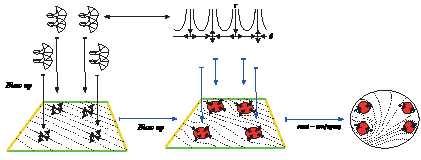
\includegraphics[width=13cm]{../assets/2155/Katok-Przyticki_example2.pdf}
\caption{Surgery on an Anosov map} \label{surgery Anosov}
\end{center}
\end{figure}

We start with the Anosov map $A(x,y)= (13\cdot x+8\cdot y, 8\cdot x+5\cdot y)$ which acts on the torus $\T^2:= \R^2/\Z^2$ endowed with the symplectic form $\Omega=dx\wedge dy$. Let $R\in O_2(\R)$ and $\lambda>0$ be such that $A= R^{-1}\times \diag (\exp (\lambda), \exp(-\lambda)) \times R $.
The set $\cP:= \{0, (1/2, 0), (0,1/2),(1/2,1/2)\}$ is formed by four fixed points of the Anosov map~$A$.

\cref{thm blow-up2} states the existence of a symplectic blow-up $p: \hat \T^2 \to \T^2 $ at $\cP$ and a lifting $\hat A\in \Diff^\omega_\Omega(\hat \T^2)$:
\[p\circ \hat A= A\circ p.\]
Moreover, there are coordinates $\hat \psi: \A(\delta)\times \cP \to \hat V$ of a neighborhood $\hat V$ of $p^{-1}(\cP)$,
a function $\Lambda\in C^\omega([0,\tfrac12 \delta^2) \times \cP,\R)$ with positive first derivative
and a Hamiltonian $\widehat H\in C^\omega (\A(\delta)\times \cP, \R)$ with time-one map $\hat \phi_H^1$ satisfying:
\[\hat A \circ \hat \psi(\theta, r,P) = \hat \psi(\phi_H^1(\theta,r,P), P) \qand \widehat H (r,\theta,P)= \Lambda (r \cdot \sin(2\theta),P), \]
for every $(\theta,r,P)$ nearby $\R/2\pi \Z\times \{0\}\times \cP$.
Note that $\hat \T^2$ is diffeomorphic to the torus without four disks. Let us precise the function $\hat H$ and $\hat \psi$ given by \cref{thm blow-up2}.
For $\delta>0$ sufficiently small, the following is a diffeomorphism onto a neighborhood $V$ of~$\cP$:
\[
\varphi: (x,y,P)\in \D(\delta)\times \cP \mto
P+R(x,y)\in V\subset \T^2.
\]
Observe that $\varphi^{-1} \circ A\circ \varphi $ coincides with the time-one of the flow of $H: (x,y,P)\in \D(\delta)\times \cP\mto \lambda \cdot x\cdot y$. Then $\hat \T^2$ is given by gluing
$\A(\delta)\times \cP$ and
$\T^2\setminus \cP$ at the open subsets $ \mathring\A(\delta)\times \cP $ and $ V \setminus \cP$ with
\begin{equation}\label{eq psi3}\psi: (\theta,r,P)\in\mathring\A(\delta) \times \cP \mto \varphi\bigl(\sqrt{2r } \cdot \cos (\theta), \sqrt{2r }\cdot \sin (\theta),P\bigr)\in V \setminus \cP.\end{equation}
Hence with $\hat \psi: \A(\delta)\times \cP \hookrightarrow \hat \T^2$ the canonical inclusion onto a neighborhood $\hat V:= p^{-1}(V)$ of the boundary of $ \hat \T^2$, we have that $\hat \psi ^{-1} \circ \hat A\circ \hat \psi$ coincides with the time-one map of the Hamiltonian:
\begin{equation}\label{def:H} \widehat H: (\theta,r,P)\in \A(\delta)\times \cP\mto \lambda\cdot r \cdot \sin(2\theta).\end{equation}

\subsection{A stochastic dynamics on the sphere with four holes}\label{S32}
In this subsection we are going to construct
an analytic and symplectic non-uniformly hyperbolic dyna\-mics~$g$ of the sphere with fours holes $\hat \bS$ as in \cref{global}. In order to do so, we proceed as depicted in \cref{surgery Anosov} [center-right], by taking the quotient of $\hat \T^2$ by an involution~$\Gamma$ that we shall define.

We recall that $\hat \T^2$ is the quotient of the disjoint union of
$\A(\delta)\times \cP $ with $\T^2\setminus \cP$ and the involution induced by the map $\psi$ of \cref{eq psi3}.
We identity $\A(\delta)\times \cP $ and $\T^2\setminus \cP$ to open subsets of $\hat \T^2$, using the projection $p$ whose restriction to each latter set is an embedding.
Recall that in this identification, $\hat A$ acts on $\T^2\setminus \cP$ as $A$ and its restriction to $\A(\delta)\times \cP $ coincides with the time-one map of the Hamiltonian $H(\theta, r, P)= \lambda\cdot r \cdot \sin(2\theta)$.

The involution $-\id$ on $\T^2$ fixes each point of $\cP$ and lifts to $\hat \T^2$ as the involution $\Gamma$ whose restriction to $\T^2\setminus \cP$ is equal to $-\id $ and whose restriction to $ \A(\delta)\times \cP $ is
\[(\theta,r,P)\in \R/2\pi \Z \times [0,\delta)\times
\cP \mto (\theta+\pi,r,P).
\]
Note that $\Gamma$ is an analytic symplectomorphism which leaves invariant the subsets $\T^2\setminus \cP$ and
$ \A(\delta)\times \cP $ of $\hat \T^2$ and
acts freely on them. Thus $\pi_\Gamma:= \hat \T^2\to \hat \T^2/\Gamma$ is a $2$-covering.
Observe that $\hat \bS:=\hat \T^2/\Gamma$ is a sphere without four holes.
As $A\circ (-\id)=-A$ and $\widehat H(\theta+\pi,r,P)=\widehat H(\theta,r,P)$, we have $\hat A\circ \Gamma=\Gamma\circ \hat A$.

Using \cref{gluing} and \cref{gluing_coro} with $O=M=\hat \bS$ and $J=\Gamma$, it comes that $\hat \bS = \hat \T^2/\Gamma$ has a canonical structure of symplectic and analytic surface for which
the $2$-covering $\pi_\Gamma $ is symplectic and analytic. Moreover the dynamics $\hat A$ descends to an analytic and symplectic dynamics $g $ on $\hat \bS $. In other words, there is $g \in \Diff^\omega_\Omega (\hat \bS)$ such that:
\[g \circ \pi_\Gamma = \pi_\Gamma \circ \hat A.\]
As the hyperbolic map $\hat A|\T^2\setminus \cP$ is a lifting of $g | \bS \setminus \partial \bS $, the map $g$ has positive metric entropy.
Let us now describe the dynamics of $g$ at the neighborhood of $\partial \bS$.
Let \[\A_\Gamma (\delta):= \R/\pi \Z \times [0, \delta)\]
and note that $ \A_\Gamma (\delta)\times \cP$ is equal to the quotient $\A(\delta)\times \cP/\Gamma$. Denote also by $H $ the analytic function such that $\widehat H=H\circ \pi_\Gamma$, which is:
\begin{equation} \label{HS}
H:= (\theta,r,P)\in \A_\Gamma (\delta)\times \cP \equiv \R/\pi \Z \times [0, \delta)\times \cP\mto \lambda\cdot r \cdot \sin(2\theta)\in \R.\end{equation}
Note that there is a $C^\omega$-symplectomorphism
$\psi_\Gamma$ from $\A_\Gamma (\delta)\times \cP $ onto the neighborhood $V_\Gamma:=\hat V/\Gamma$ of the boundary $\partial \hat \bS $ such that $\psi_\Gamma\circ \pi_\Gamma= \hat \psi$. Moreover $ \psi_\Gamma^{-1} \circ g \circ \psi_\Gamma$
coincides with the time-one map of the flow of $H $. To summary we obtained:

\begin{claim}\label{fonda1} There is a symplectic sphere with four holes $(\hat \bS, \Omega)$ and $g\in \Diff^\omega_\Omega(\hat \bS)$ such that:
\begin{enumerate}
\item\label{fonda11} every point $x\in\hat \bS$ has positive Lyapunov exponent: $\limsup \frac1n \log \|Dg^n\| \to \infty$,
\item\label{fonda12} there are $\delta>0$ and a $C^\omega$-symplectomorphism
$ \psi_\Gamma$ from $\A_\Gamma (\delta)\times \cP$ onto a
neighborhood of $\partial \hat \bS\subset \hat \bS$, such that $g$ coincides with the time-one map of the Hamiltonian flow of $H_\Gamma:= H\circ \psi_\Gamma^{-1}$ at a neighborhood of $\partial \hat \bS$.
\end{enumerate}
\end{claim}

\subsection{Integrable cap}\label{S33}
We are now going to construct the cap which recaps the holes of $\hat \bS$. For $\epsilon>0$, let
\[\A_\Delta (\epsilon)= \R/\pi \Z \times (-\epsilon, 0]\]
and denote also $H:= (\theta,r)\in \A_\Delta(\delta) \mto \lambda\cdot r\cdot \sin(2\theta)$. We will see in the next subsection that the following claim provides the sought cap:

\begin{claim}\label{fonda2}
There exist a $C^\omega$-Hamiltonian $H_\Delta$ on a closed symplectic disk $(\Delta,\Omega) $ which satisfies:
\begin{enumerate}
\item\label{fonda21} $H_\Delta$ has only two critical points in $\Delta\setminus \partial \Delta $, the Hessian is definite positive at them,
\item\label{fonda22} there are $\epsilon\in (0,\tfrac12 \delta^2)$ and a $C^\omega$-symplectomorphism
$ \psi_\Delta$ from $ \A_\Delta (\epsilon)$ onto a
neighborhood $V_\Delta$ of the boundary of $\Delta$
such that $H= H_\Delta\circ \psi_\Delta$.
\end{enumerate}
\end{claim}

In this subsection we show this claim, by proceeding as in \cref{cap surgery}.

\begin{figure}[htb]
\begin{center}
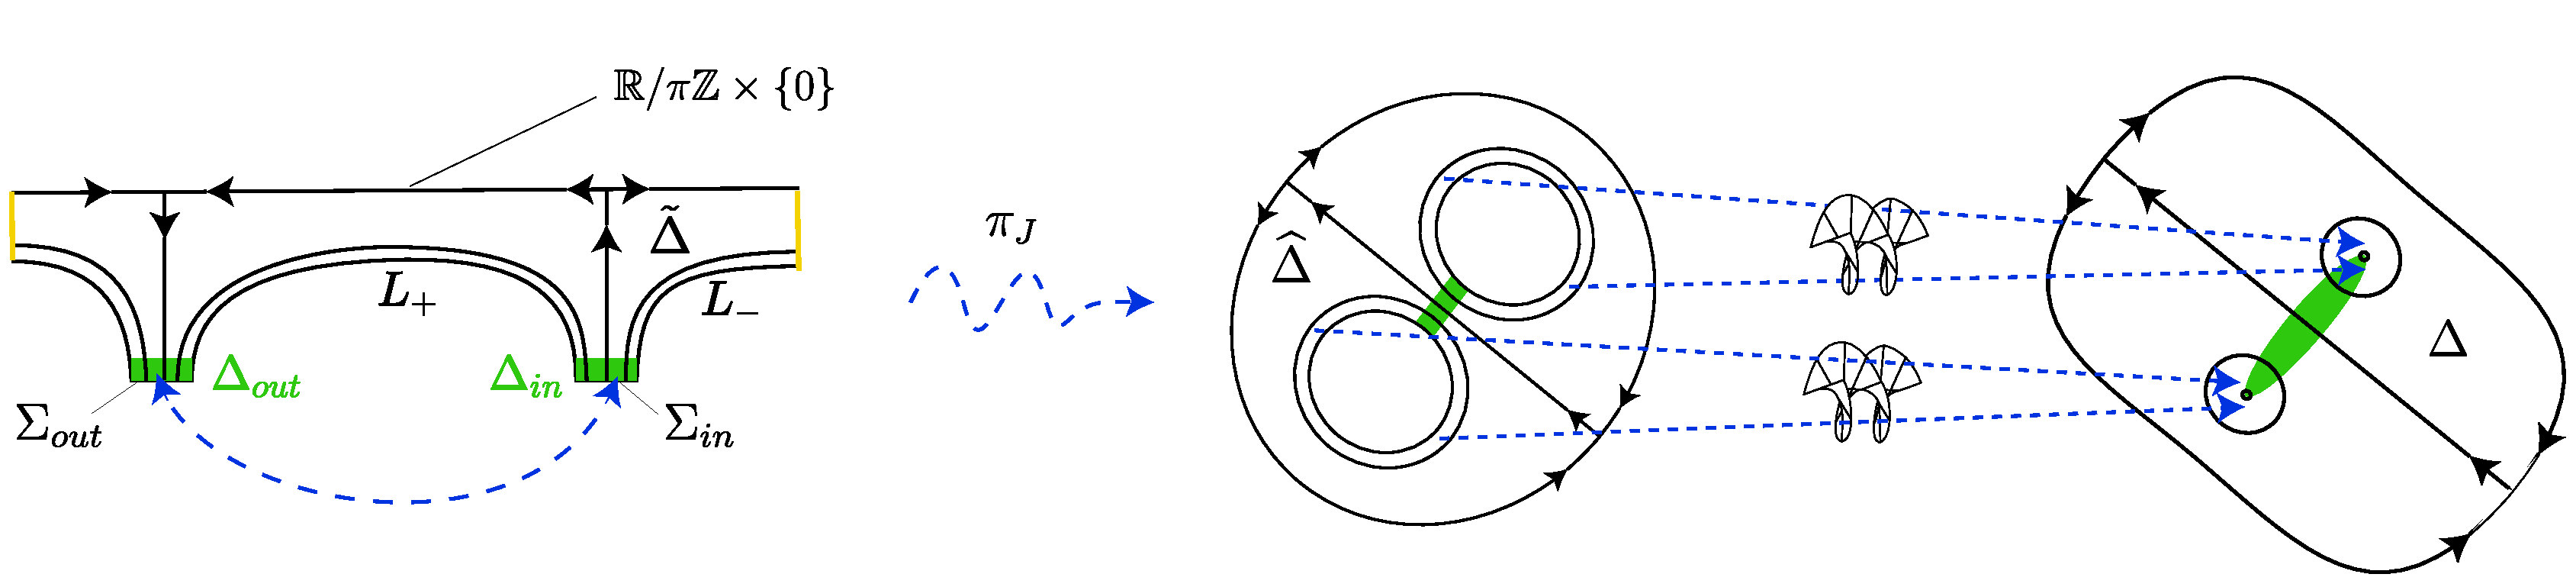
\includegraphics[width=13cm]{../assets/2155/cap_surgery.pdf}
\caption{Making an integrable cap by gluing the green rectangles together and then blowing down.} \label{cap surgery}
\end{center}
\end{figure}

First we shall define $\tilde \Delta\subset \A_\Delta(\delta)$ as in \cref{cap surgery} [left]. For a small $\epsilon\in(0,\delta)$ fixed later, we put:
\[\tilde \Delta:= \big\{(\theta,r)\in \R/\pi\Z\times
(-\epsilon, 0]: |H(\theta,r)| \le \epsilon^2 \big\}.\]
Now fix $\epsilon>0$ small enough so that the set $\cl(\tilde \Delta)$ is a pentagon whose sides are $\R/\pi\Z\times \{0\}$, $L_+$, $L_-$, $\Sigma_\mathrm{in}$ and $\Sigma_\mathrm{out}$, where:
\begin{align*}
L_+&:=\{ (\theta,r)\in \R/\pi\Z \times (-\epsilon, 0): H(\theta,r)= \epsilon^2\},\\
\quad L_-&:=\{ (\theta,r)\in \R/\pi\Z\times (-\epsilon, 0): H(\theta,r)= - \epsilon^2\},\\
\Sigma_\mathrm{in}&:= \{ \theta\in (-\pi/4, \pi/4): |H(\theta,-\epsilon)|\le \epsilon^2\}\times \{-\epsilon\} \\
\tag*{and}
\Sigma_\mathrm{out}&:=\{ \theta\in (\pi/4, 3\pi/4): | H(\theta,-\epsilon)|\le \epsilon^2\}\times \{-\epsilon\}.
\end{align*}

Let $(\phi^t)_t$ be the flow of $H$; observe that $\partial_t \phi^t:= \lambda(-\sin(2\theta), 2\cdot r\cdot \cos(2\cdot \theta))$ is tangent to the sides of $\R/\Z\times \{0\}$, $L_+$ and $L_-$.
On the other hand, it enters into $\tilde \Delta$ by $\Sigma_\mathrm{in}$ and exits $\tilde \Delta$ by $\Sigma_\mathrm{out}$. Indeed, we have:
\begin{align*}
\Sigma_\mathrm{in}&:= \left[- \tfrac12 \arcsin\left(\sfrac \epsilon\lambda \right),\tfrac12 \arcsin\left(\sfrac \epsilon\lambda \right)\right]\times \{-\epsilon\}\\
\tag*{and}
\Sigma_\mathrm{out}&:= \left[\sfrac\pi2 - \tfrac12 \arcsin\left(\sfrac \epsilon\lambda \right),\sfrac\pi2 +\tfrac12 \arcsin\left(\sfrac \epsilon\lambda \right)\right]\times \{-\epsilon\},
\end{align*}
and on these segments, the $r$-component of $ \partial_t \phi^t(\pi/2, r)|_{t=0}$ is equivalent (as $\epsilon$ is small) to \resp $2\lambda \cdot \epsilon$ and $-2\lambda \cdot \epsilon$.
As in \cref{cap surgery} [left], we glue $\tilde \Delta$ to itself at:
\[
\Delta_\mathrm{in}\sqcup \Delta_\mathrm{out}\quad \text{with }
\Delta_\mathrm{in}:=
\bigcup_{0< t<1} \phi^{t}(\Sigma_\mathrm{in}) \subset \tilde \Delta \qand \Delta_\mathrm{out}
:= \bigcup_{0< t<1} \phi^{-t}(\Sigma_\mathrm{out}) \subset \tilde \Delta,
\]
using the involution $J$ which sends $\phi^{t}(\theta, -\epsilon)\in \Delta_\mathrm{in}$ to $\phi^{t-1}(\pi/2-\theta, -\epsilon)\in \Delta_\mathrm{out}$ and vice-versa for every $t\in (0,1)$. Note that we can use \cref{gluing} with $M=\tilde \Delta$ and $O:= \Delta_\mathrm{in}\sqcup \Delta_\mathrm{out}$ since condition \eqref{enum:C} is satisfied with the following neighborhood of $\cl(O)\setminus O \subset \tilde \Delta$:
\begin{align*}
W&:=W_\mathrm{in}\sqcup W_\mathrm{out},\\
\tag*{where}
W_\mathrm{in}
&:= \bigcup_{\sfrac12 <t<2} \phi^t(\Sigma_\mathrm{in}) \subset \tilde \Delta
\qand
W_\mathrm{out}:= \bigcup_{\sfrac12 <t<2} \phi^{-t}(\Sigma_\mathrm{out})\subset \tilde \Delta.
\end{align*}
Using that $J$ is symplectic and leaves $H$ equivariant ($H\circ J|O= H|O$), \cref{gluing} and \cref{gluing_coro} asserts that the quotient $\widehat \Delta:= \tilde \Delta/J$ has a unique structure of $C^\omega_\Omega$\nobreakdash-surface for which $\pi_J: \tilde \Delta\to \widehat \Delta$ is of class $C^\omega_\Omega$ and for which there exists $\widehat H\in C^\omega(\tilde \Delta, \R)$ satisfying:
\[\widehat H\circ \pi_J= H.\]
We notice that $\widehat \Delta$ is symplectomorphic to a closed disk $\bar D$ without two open disks $\D_+$ and $\D_-$, as depicted in \cref{cap surgery} [center]:
\[\widehat \Delta= \bar D \setminus (\D_+ \sqcup \D_-).\]
We chose the identification such that the circle $\partial \D_\pm $ is the quotient of $L_\pm$ for each $\pm\in\{ -,+\}$ and the circle $\partial \bar D $ is the quotient of $\R/\pi \Z\times \{0\}$.

As the symplectic gradient of $H$ is colinear to $\R/\pi \Z\times \{0\}$ and $L_\pm$, and moreover non-degenerate at $\tilde \Delta\setminus \R/\pi \Z\times \{0\}$, the same occurs for the quotient: the symplectic gradient of $\widehat H$ is colinear to the boundary $\partial \widehat \Delta$ and non-degenerate on $D\setminus (\D_+\sqcup \D_-)$.

Hence we can apply \cref{thm blow-down} twice to blow down each of the holes of $\widehat \Delta$. This
defines a symplectic closed disk $\Delta$ and a $C^\omega$-map $p: \widehat \Delta\to \bar \Delta$ so that
$p$ sends $\partial \D^+\sqcup \partial \D^-$ to two points $\{p_+,p_-\} \subset \Delta$ and the restriction $p|\widehat \Delta \setminus (\partial \D^+\sqcup \partial \D^-)$ is a symplectomorphism onto $\widehat \Delta \setminus \{p_+,p_-\}$. Moreover, \cref{thm blow-down} implies that there is a $C^\omega$-Hamiltonian $H_\Delta$ on $\Delta$ such that $H_\Delta\circ p= \widehat H$ for which $p_+$ and $p_-$ are elliptic. As $\tilde H$ has no critical point, it comes that $H_\Delta$ has no critical point on $\text{int }\Delta \setminus \{p_-,p_+\}$. This gives the first statement of \cref{fonda2}. The second statement is obvious since $p$ is a symplectomorphism from a neighborhood of $\partial \bar D\subset \widehat \Delta$ onto a neighborhood of $\partial\Delta\subset \Delta$, and since $\pi_J$ is a symplectomorphism from a neighborhood of $\partial\Delta\subset \Delta$ onto a neighborhood of $\R/\pi \Z\times \{0\}$ in $\tilde \Delta$. Hence for $\epsilon>0$ sufficiently small, the restriction $\psi_\Delta:= p\circ \pi_J|\A_\delta(\epsilon)$ is a $C^\omega$-symplectomorphism onto a neighborhood $V_\Delta$ of $\partial \Delta\subset \Delta$. Moreover $H_\Delta\circ \psi_\Delta = H$.\enlargethispage{.5\baselineskip}%

\subsection{Gluing the cap $\Delta$ to a hole of $\hat \bS$}\label{S34}
In this subsection we show the following:

\begin{claim}\label{recap}
For every $1\le n\le 4$, the symplectic and analytic surface $(\hat \bS,\Omega)$ can be extended to a symplectic and analytic surface $(\mathbb M,\Omega)$ which is the union of $\hat \bS$ and $n$-copies of the disk $\Delta$, each of which is glued at its boundary to a different component of $\partial \hat\bS$, and such that there is a $C^\omega$-symplectomorphism $f^{\mathbb M}$ of $\mathbb M$ whose restriction to~$\hat \bS$~is~$g$ and
whose restriction to each copy of $\Delta$ is the time-one map $f$ of the~Hamiltonian~$H_\Delta$.
\end{claim}

\begin{proof}
Let us show the case $n=1$. Let C be a component of $\partial \hat \bS$.
Let $P\in \cP$ be such that $V_1:=\psi_\Gamma(\A_\Gamma(\epsilon) \times \{P\})$ is a neighborhood of $C$ in $\hat \bS$ by \cref{fonda1}\eqref{fonda12}. Note that $V_2:= \psi_\Delta(\A_\Delta(\epsilon))$ is a neighborhood of $\partial \Delta $ in $\Delta$ by \cref{fonda2}\eqref{fonda22}.
To this end, it suffices to apply \cref{gluing2} with $M_1=\hat \bS$, $M_2= \Delta$, $f_1= g$, $f_2= f$ and $f_{12}$ the time-one of the Hamiltonian flow of $H: (\theta,r)\in \R/\pi \Z\times (-\epsilon, \epsilon)\mto r\sin(2\theta)$ and
\[\Phi:= V_1\sqcup V_2\to \R/\pi \Z\times (-\epsilon, \epsilon),\]
defined by $\Phi(x)=y$ iff $x= \psi_\Gamma(y,P)$ for $x=\psi_\Delta(y)$.
Note that by Claims \ref{fonda1}\eqref{fonda12} and \ref{fonda2}\eqref{fonda22}, the assumptions of \cref{gluing2} are satisfied; this theorem provides the sought conclusions.

Finally note that the case $4\ge n>1$ can be proved by induction on $n$ using the later argument of the inductive step.
\end{proof}

\section{Application of the construction}\label{S4}
\Subsection{Proof of \cref{main,coroAprime}}\label{S41}
\begin{proof}[Proof of \cref{main}. Case where $S$ is the sphere]
We apply \cref{recap} with $n=4$. Then each of the four holes of $\hat \bS$ are recapped with a copy of the disk $\Delta$, so that $\mathbb M$ is a symplectic sphere $\bS$. The claim asserts the existence of an analytic symplectomorphism~$f^{\bS}$ whose restriction to
$ \hat \bS\subset \bS$ is the stochastic map $g$ and whose restriction to the complement $ \bS\setminus \hat \bS$ is equal to four copies of the cap dynamics $h$ which displays each time two elliptic islands and so eight in total.

\subsubsection*{Proof of \cref{main}. Case where $S$ is the torus}
We apply \cref{recap} with $n=2$. Then two holes of $\hat \bS$ are recapped with two copies of the disk $\Delta$, so that $\mathbb M$ is an annu\-lus $\A$. The claim asserts the existence of an analytic symplectomorphism~$f^{\A}$ whose restriction to
$ \hat \bS\subset \A$ is the stochastic map $g$ and whose restriction to the complement $ \A\setminus \hat \bS$ is equal to two copies of the cap dynamics $f$ which displays each time two elliptic islands and so four in total. Moreover, there is an open neighborhood~$N$ of the two circles~$\partial \A$ which is symplectomorphic to $\A(\delta)\times \{+1,-1\}$, via a $C^\omega$\nobreakdash-symplectomorphism~$ \psi$ which conjugates the dynamics $f^\A|N$ to the time-one map of the Hamiltonian \hbox{$H: (\theta,r, \pm1)\mto \lambda\cdot r\cdot \sin(2\theta)$}.

So it suffices to glue the two boundaries of $\partial \A$ so that the quotiented dynamics remains analytic (and symplectic).
To this end, we apply \cref{gluing2} with $M_1=M_2=\A$, $f_1=f_2=f^\A$, $f_{12}$ the time-one map of the flow of $(\theta,r)\mto \lambda\cdot r\cdot \sin(2\theta)$ and the map $\Phi:
\psi(\A(\delta)\times \{+1,-1\})\to \R/\pi\Z \times (-\delta,\delta)$ which sends $\psi(\theta,r,\pm1)$ to $(\pm \theta, \pm r)$ for every $(\theta, r, \pm1)\in \A(\delta)\times \{+1,-1\}$.\enlargethispage{.5\baselineskip}%

\subsubsection*{Proof of \cref{main}. Case where $S$ is a surface of higher genus}
We apply \cref{recap} with $n=1$. Then $\mathbb M$ is a pair of pants $\P$: a disk with two holes. The dynamics $f^\P$ on $\P$ is of class $C^\omega_\Omega$ and is stochastic at $\hat \bS\subset \P$ and integrable at one cap $\Delta$ with exactly two elliptic islands. We recall that every closed, oriented surface $S$ of genus $\ge 2$ displays a pants decomposition. We glue canonically (using \cref{gluing2} as above) the pants at their boundaries to obtain the sought dynamics.
\end{proof}

\begin{proof}[Proof of \cref{coro isotopy} for $S$ equal to the torus and $f$ isotopic to the identity]
We constructed above a symplectic and analytic map $f^\A$ on the closed annulus $\A $ satisfying the coexistence phenomena and moreover the following property.
There is an open neighborhood $N$ of the boundary $\partial \A$ which is symplectomorphic to $\A(\delta)\times \{+1,-1\}$, via a $C^\omega$-map $ \psi$ which conjugates the dynamics $f^\A|N$ to the Hamiltonian flow of $H: (\theta,r, \pm1)\mto \lambda\cdot r\cdot \sin(2\theta)$.

In the proof of \cref{main}, we glued the two components $C_+$ and $C_-$ of $\partial \A$ to obtain a dynamics on the torus displaying the coexistence phenomena. Nevertheless this dynamics is \emph{a priori} in a non-trivial isotopy class. To vanish this isotopy class, the idea is to glue $f^\A$ with its inverse $(f^\A)^{-1}$. To this end, let $f_1$ be the dynamics induced by $f^\A$ on the copy
$M_1=\A\times \{1\}$ of $\A$, and let $f_2 $ be the dynamics induced by $(f^\A)^{-1}$ on another copy
$M_2=\A\times \{-1\}$ of $\A$.

At the boundary $C_+\sqcup C_-$ of $\A$, the map $(f^\A)^{-1}$ is conjugated via $\psi$ to the time-one map of the flow of $-H(\theta, r,\pm1)= H(-\theta -\pi/2, -r,\pm1)$. So we can apply \cref{gluing2} to glue $M_1$ and $M_2$ at $C_+\times \{1\}$ and $C_+\times \{-1\}$ with the following map:
\begin{align*}
\Phi_+: \psi(\A(\delta)\times \{1\})\times \{-1,1\}&\to \R/\pi\Z\times (-\delta,\delta)\\
(\psi(r,\theta,1),\pm1) &\mto (\pm \theta+(\pm1-1)\pi/4,\pm r).
\end{align*}
Similarly the gluing is done at $C_-\times \{1\}$ and $C_-\times \{-1\}$ with the following map:
\begin{align*}
\Phi_-:\psi(\A(\delta)\times \{-1\})\times \{-1,1\}&\to \R/\pi\Z\times (-\delta,\delta)\\
(\psi(r,\theta,-1),\pm1) &\mto (\pm \theta+(\pm1-1)\pi/4,\pm r).
\end{align*}
Then observe that the surface obtained after these two gluings is a symplectic torus endowed with a $C^\omega_\Omega$-dynamics $f$ whose restriction to the halve of this torus is $f^\A$ and to other other halve is $(f^\A)^{-1}$. Hence $f$ displays the coexistence phenomena and is isotopic to the identity (as the twist of $(f^\A)^{-1}$ vanishes the one of $f^\A$).
\end{proof}
\begin{proof}[Proof of \cref{coroAprime}]
We apply \cref{recap} with $n=3$. This defines an analytic and symplectic map $f^\D$ on the disk $\D$. Note that the disk is not endowed with its standard symplectic form, but using \cite{DM90}, we can analytically conjugate it to one which leaves invariant the standard symplectic form on $\D$. The image $\cI$ of $\hat \bS$ in $\D$ is depicted \cref{fig:island}. Therein the Lyapunov exponent function $\Lambda$ is equal to a positive constant.
\begin{figure}[htb]
	\centering
		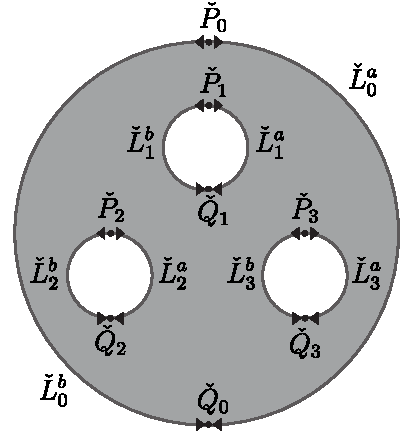
\includegraphics[width=5cm]{../assets/2155/EXAMPLEFIG.pdf}
\caption{Stochastic island $\cI$ in grey.}\label{fig:island}
\label{fig:oldcoord}
\end{figure}
In the sense of \cite{BT19} (inspired from \cite{Ka79, AP09,Pr82}), the set $\cI$ is called a \emph{stochastic island}. This means that $\cI$ is a disk with three holes; and that the boundary of $\cI$ is formed by four pairs of heteroclinic bi-links $\{(\check L_i^a, \check L^b_i): 0\le i\le 3\}$. Each $\check L_i^a\cup \check L_i^b$ is a smooth circle included
in the stable and unstable manifolds of hyperbolic fixed points $\check P_i$ and $\check Q_i$ respectively:
\[\check L_i^a\cup \check L_i^b \subset W^u(\check P_i; f^\D)\cup W^s(\check Q_i; f^\D).\]
For every $f$ which is $C^1$-close to $f^\D$, for every $0\le i\le 3$, the \emph{hyperbolic continuations} $P_i$ and $Q_i$ of $\check P_i$ and $\check Q_i$ are uniquely defined hyperbolic fixed points for $f$. If $\{W^u(P_i; f)\cup W^s(Q_i;f): 0\!\le\! i \!\le\! 3\}$ form four heteroclinic bi-links $\{L_i^a\cup L^b_i: 0\!\le\! i\!\le\! 3\}$ close to $\{\check L_i^a\cup \check L^b_i: 0\le i\le 3\}$, then we say that the \emph{bi-links are persistent for the perturbation $f$}.

Then the next proposition implies \cref{coroAprime}.
\end{proof}
\begin{proposition}[{\cite[Prop.\,2.1]{BT19}}]\label{KPAP}
For every conservative map $f$ which is $C^2$\nobreakdash-close to $f^\D$ if the bi-links are persistent, then the continuations of these bi-links bound a stochastic island. In particular, the metric entropy of $f$ is positive.
\end{proposition}
\subsection{Proof of \cref{coro isotopy}}\label{S42}
To achieve the proof of \cref{coro isotopy}, it remains the case of mappings isotopic to pseudo-Anosov maps (the case of the torus has been done above and the case of the sphere is an immediate consequence of \cref{main}). To carry them we use the following generalization of the cap's construction:
\begin{proposition}\label{generalized cap}Let $(S,\Omega)$ be a symplectic surface and let $f\in \Diff^\omega_\Omega(S)$ be displaying a periodic hyperbolic orbit with positive eigenvalues.
Let $(\hat S,\omega)\to (S, \Omega)$ be the blow up given by \cref{thm blow-up2} and let $\hat f\in \Diff^\omega_\Omega(\hat M)$ be the lifting of $f$.

Then there is an analytic extension $(\tilde S,\Omega)\supset (\hat S,\Omega)$ and an extension $\tilde f\in \Diff^\omega_\Omega(\tilde S)$ of $\hat f$ such that $\tilde S$ is diffeomorphic to $S$ and $\tilde S\setminus \hat S$ consists of a finite union of disks on which $\tilde f$ is the product of a cycle $k\in \Z/n\Z\to k+1$ with an integrable map of the disk displaying three elliptic fixed points.
\end{proposition}
This proposition is proved below.
\begin{proof}[Proof of \cref{coro isotopy} for $f$ isotopic to a pseudo-Anosov map.]
Let $(S, \Omega)$ be a symplectic orientable, closed surface. Then by \cite{GK82,Ge85}, any orientation preserving pseudo-Anosov isotopy class is represented by an analytic symplectomorphism $f$. Then observe that \cref{coro isotopy} follows immediately from
\cref{generalized cap} and the next lemma. \end{proof}
\begin{lemma}
The map $f$ displays a hyperbolic periodic cycle $(P_i)_{i\in \Z_q}$ with positive eigenvalues.\end{lemma}
\begin{proof}
As $f$ has positive topological entropy, it displays a horseshoe \cite{Ka80} with at least two rectangles. There are two possibilities:
Either one of these rectangles is not rotated by the induced dynamics, and so we get immediately a saddle periodic cycle with positive eigenvalues. Or both rectangle are rotated by a half turn. Then we can compose the induced dynamics by these two rectangles to obtain a hyperbolic periodic orbit with positive eigenvalues.
\end{proof}

\begin{proof}[Proof of \cref{generalized cap}]
Let $\cP$ be the periodic orbit which is blown up and let $p: \hat S\to S$ be the canonical projection. By \cref{thm blow-up2}, there are coordinates $\hat \psi: \A(\delta)\times\nobreak \cP \to \hat V$ of a neighborhood $\hat V$ of $p^{-1}(\cP)$ and a Hamiltonian $H\in C^\omega (\A(\delta)\times\nobreak \cP, \R)$ whose time-one map $\phi_H^1$ satisfies:
\[\hat f \circ \hat \psi (\theta, r,P) = \hat \psi(\phi_H^1(\theta,r,P), f(P)) \qand H (r,\theta,P)= \Lambda (r \cdot \sin(2\theta)) \]
for every $(\theta,r,P)$ nearby $\R/2\pi \Z\times \{0\}\times \cP$
and for a function $\Lambda\in C^\omega([0,\tfrac12 \delta^2),\R)$ with positive first derivative.
Note that $\Lambda$ does not depend on $P \in \cP$ because $\cP$ is formed by a unique orbit.
Hence on $\hat V$ the dynamics is conjugated to the product of the shift map on $\cP$ with the time-one map $f_o$ of the Hamiltonian flow of:
\[H_o: (r,\theta)\in \A(\delta)=\R/2\pi\Z\times [0,\tfrac12 \delta^2)\mto \Lambda (r \cdot \sin(2\theta)). \]

Observe that on $C= \R/2\pi\Z\times \{0\}$, the flow of $H_o$ displays four saddle fixed points $Q_q=((\sfrac q 2+1)\sfrac\pi4,0)$ with $q\in \Z/4\Z$, so that $ \bigcup_{i=1}^2 W^s(Q_{2i})\cup \{Q_{2i+1}\} =
\bigcup_{i=1}^2 W^u(Q_{2i+1})\cup \{Q_{2i}\}= C$.
In particular $C$ consists of four heteroclinic links. Note also that $H_o$ can be canonically extended to $\R/2\pi \Z\times (-\tfrac12 \delta^2,\tfrac12 \delta^2)$. Thus we can use the next lemma with $k=2$ to recap each hole of $\hat S$ (as we did in \cref{recap}) of $\hat S $ and obtain the sought surface and dynamics (more precisely the extension is $ \cP\times\Delta$ endowed with the product of shift map on $\cP$ with the time-one map of the Hamiltonian $H_\Delta$ defined in the next lemma). \end{proof}

\begin{lemma}[Generalized cap]\label{fonda3}\label{Generalized cap}
Let $\delta>0$ and let $H_o$ be an analytic Hamiltonian defined on $ \R/2\pi\Z\times (-\tfrac12 \delta^2,0]$ such that $C=\R/2\pi\Z\times \{0\} $ is a union of $2k$-heteroclinic links:
\[C= \bigcup_{i\in \Z_k} W^s(Q_{2i}) \cup \{Q_{2i+1}\}= \bigcup_{i\in \Z_k} W^u(Q_{2i+1}) \cup \{Q_{2i}\}.\]
Then there exist a $C^\omega$-Hamiltonian $H_\Delta$ on a symplectic disk $(\Delta,\Omega) $ such that:
\begin{enumerate}
\item $H_\Delta$ has only $k+1$ critical points, their Hessian is definite positive,
\item there are $\epsilon\in (0,\tfrac12 \delta^2)$ and a $C^\omega$-symplectomorphism $ \psi_\Delta$ from $ \R/2\pi\Z \times (-\epsilon,0]$ onto a neighborhood $V_\Delta$ of the boundary of $\Delta$
such that $H_o= H_\Delta\circ \psi_\Delta$.
\end{enumerate}
\end{lemma}

\begin{proof} We depict the construction for $k=2$ in \cref{cap surgeryS} [left-center]. For $k=1$, this lemma implies \cref{fonda2}; its proof is basically the same.
\begin{figure}[htb]
\begin{center}
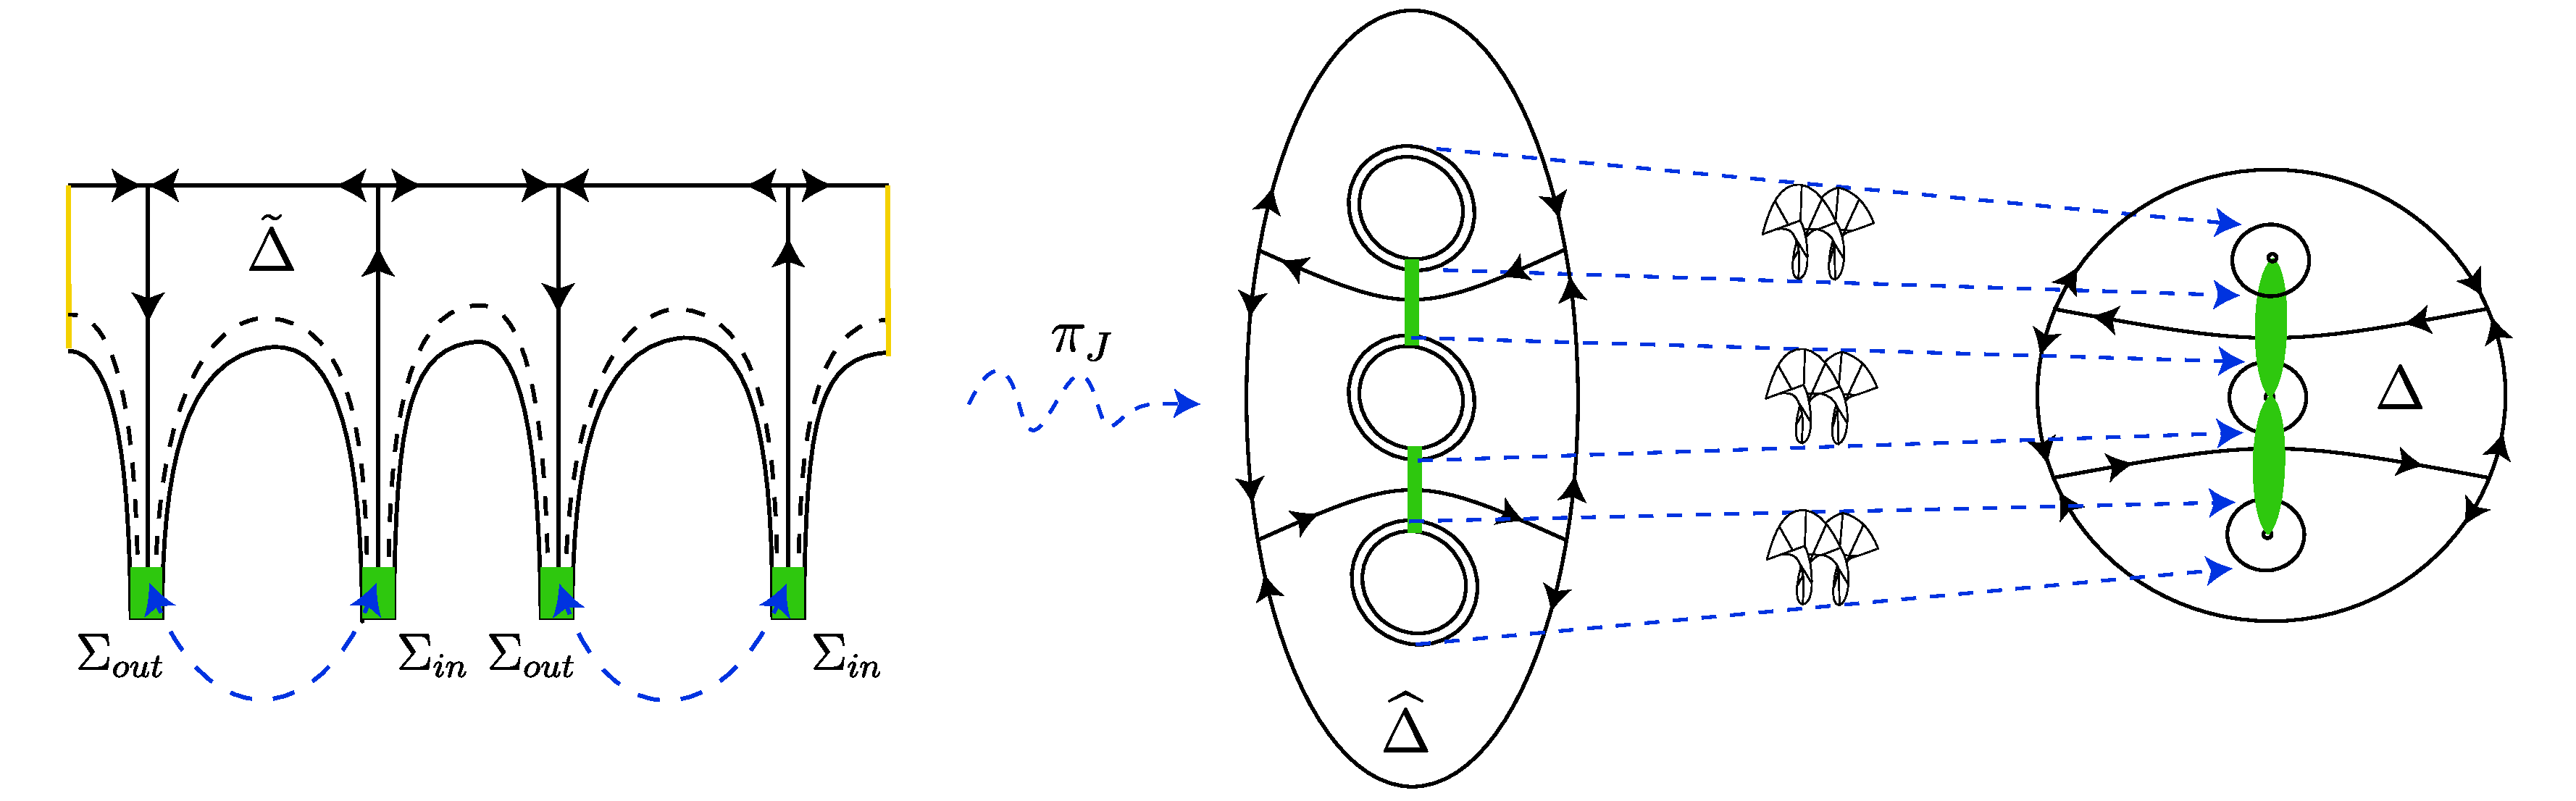
\includegraphics[width=13cm]{../assets/2155/cap_surgeryS.pdf}
\caption{Making an integrable generalized cap by surgery with $k=2$.} \label{cap surgeryS}
\end{center}
\end{figure}

On $C$ the function $H_o$ must be constant; let us assume it equal to $0$. For $\eta>0$ small, we define:
\[\tilde \Delta:= \{(\theta,r)\in \R/2\pi\Z\times
(-\epsilon, 0]:
|H_o(\theta,r)|\le \epsilon^2 \}.\]
The boundary of $\cl(\tilde \Delta) $ is made by $4k+1$ curves (see \cref{cap surgery} [left]); $2k$ of them form the components of:
\[\Sigma:=\{\theta\in \R/2\Z:
|H_o(\theta,-\epsilon)|\le \epsilon^2 \}\times \{-\epsilon\}.\]
Indeed, $H_o$ has critical point only at $\{Q_i:1\le i\le 2k\}$, which are non degenerate, so $\Sigma$ is indeed formed by $2k$-components, each of which with length $\asymp \epsilon$ when $\epsilon\to 0$. Note that:
\[\Sigma= \Sigma_\mathrm{out}\sqcup \Sigma_\mathrm{in},\quad \text{with } \Sigma_\mathrm{out}= \bigsqcup_{i\in \Z_k} \Sigma_{\mathrm{out},i}\qand
\Sigma_\mathrm{in} = \bigsqcup_{i\in \Z_k} \Sigma_{\mathrm{in},i},\]
and where each $\Sigma_{\mathrm{out},i}$ is the component of $\Sigma$ which intersects $W^u_{2\eta}(Q_{2i})$ while each $\Sigma_{\mathrm{in},i}$ is the component of $\Sigma$ which intersects $W^s_{2\eta}(Q_{2i+1})$. On each $\Sigma_{\mathrm{out},i}$, the restriction $H_o|\Sigma_{\mathrm{out},i}$ is a diffeomorphism onto $[-\epsilon^2,\epsilon^2]$. Thus there is a canonical parametrization of $\Sigma_\mathrm{out}$ with $[-\epsilon^2,\epsilon^2]\times \Z_k$. Likewise there is a canonical parametrization of $\Sigma_\mathrm{in}$ with $[-\epsilon^2,\epsilon^2]\times \Z_k$. Let $\phi^t$ be the Hamiltonian flow of $H_o$.
As in \cref{cap surgeryS} [left-center], using \cref{gluing} as in \cref{fonda2}, we glue $\tilde \Delta$ to itself at:
\[
\Delta_\mathrm{out}\sqcup \Delta_\mathrm{in}\quad \text{with }
\Delta_\mathrm{out}:=
\bigcup_{t\in (0,1)} \phi^{-t}(\Sigma_\mathrm{out}) \subset \tilde \Delta \qand \Delta_\mathrm{in}
:= \bigcup_{t\in (0,1)} \phi^t(\Sigma_\mathrm{in}) \subset \tilde \Delta,
\]
using the $C^\omega_\Omega$-involution $J$ which swap for every $t\in (0,1)$ and $k\in \Z_k$,
each pair of points $\phi^{-t}(\theta_0, -\epsilon)$ and $\phi^{1-t}(\theta'_0, -\epsilon)$ among $(\theta_0, -\epsilon)\in \Sigma_{\mathrm{out},k}$ and $(\theta'_0, -\epsilon)\in \Sigma_{\mathrm{in},k}$ such that $H_o(\theta_0,-\epsilon)= H_o(\theta'_0,-\epsilon)$.
Then \cref{gluing} and \cref{gluing_coro} assert that the quotient $\widehat \Delta:= \tilde \Delta/J$ has a unique structure of $C^\omega_\Omega$-surface for which $\pi_J: \tilde \Delta\to \widehat \Delta$ is of class $C^\omega_\Omega$. Moreover as $J$ leaves $H_o$ equivariant, there exists $\widehat H\in C^\omega(\tilde \Delta, \R)$ satisfying:
\[\widehat H\circ \pi_J= H_o.\]
We notice that $\widehat \Delta$ is equal to the closed disk $\bar \D$ without $k+1$ disks $(\D_i)_{0\le i\le k}$ as depicted in \cref{cap surgeryS} [center]:
\[\widehat \Delta= \bar \D \setminus \Bigl(\bigcup_{i=0}^k \D_i\Bigr).\]
Also on $\partial \D_i$, the Hamiltonian $\widehat H$ is equal to $\epsilon^2$ or $-\epsilon^2$. Hence the symplectic gradient of $\widehat H$ is colinear to each boundary $\partial \D_i$. Moreover its symplectic gradient does not display critical point at these circles.
So we can blow down each of the $k+1$-holes $\D_i$ using \cref{thm blow-down} as depicted in \cref{cap surgeryS} [center-right]. These blow-downs define a symplectic closed disk $(\Delta,\Omega)$ endowed with an analytic Hamiltonian $H_\Delta$ satisfying the second item of the lemma. As the unique critical points of $H_o|\tilde \Delta$ were $(Q_i)_{i\in \Z_{2k}}$, these surgeries create only $k+1$-new critical points at $P_i$ which are all with definite positive Hessian.
\end{proof}

% End literal retained input author-body.tex

\begin{thebibliography}{99}
\bibitem{AKN88} V. I. Arnol’d, V. V. Kozlov \& A. I. Neĭshtadt - Dynamical systems. III , Encyclopaedia of Math. Sciences , vol. 3 , Springer-Verlag, Berlin, 1988
\bibitem{AP09} A. Arroyo \& E. Pujals - “${C}^k$-robust transitivity for surfaces with boundary” , 2009
\bibitem{Ar19} M.-C. Arnaud - “La démonstration de la conjecture de l’entropie positive d’Herman d’après Berger et Turaev” , in Séminaire Bourbaki , Astérisque , vol. 430 , Société Mathématique de France, Paris, 2021, p. 1-26
\bibitem{burns_gerber_1989} K. Burns \& M. Gerber - “Real analytic Bernoulli geodesic flows on $S^2$” , Ergodic Theory Dynam. Systems 9 (1989) no. 1, p. 27-45
\bibitem{Bo67} N. Bourbaki - Éléments de mathématique. Fasc. XXXIII. Variétés différentielles et analytiques. Fascicule de résultats (Paragraphes 1 à 7) , Actualités Scientifiques et Industrielles , vol. 1333 , Hermann, Paris, 1967
\bibitem{BT19} P. Berger \& D. Turaev - “On Herman’s positive entropy conjecture” , Adv. Math. 349 (2019), p. 1234-1288
\bibitem{DM90} B. Dacorogna \& J. Moser - “On a partial differential equation involving the Jacobian determinant” , Ann. Inst. H. Poincaré Anal. Non Linéaire 7 (1990) no. 1, p. 1-26
\bibitem{Donnay} V. Donnay - “Geodesic flow on the two-sphere. I. Positive measure entropy” , Ergodic Theory Dynam. Systems 8 (1988) no. 4, p. 531-553
\bibitem{Ge85} M. Gerber - Conditional stability and real analytic pseudo-Anosov maps , Mem. Amer. Math. Soc. , vol. 54, no. 321 , American Mathematical Society, Providence, RI, 1985
\bibitem{GK82} M. Gerber \& A. Katok - “Smooth models of Thurston’s pseudo-Anosov maps” , Ann. Sci. École Norm. Sup. (4) 15 (1982) no. 1, p. 173-204
\bibitem{Go12} A. Gorodetski - “On stochastic sea of the standard map” , Comm. Math. Phys. 309 (2012) no. 1, p. 155-192
\bibitem{He98} M. Herman - “Some open problems in dynamical systems” , Doc. Math. (1998), p. 797-808, Proceedings ICM (Berlin, 1998), Extra Vol. II
\bibitem{Ka79} A. Katok - “Bernoulli diffeomorphisms on surfaces” , Ann. of Math. (2) 110 (1979) no. 3, p. 529-547
\bibitem{Ka80} A. Katok - “Lyapunov exponents, entropy and periodic orbits for diffeomorphisms” , Publ. Math. Inst. Hautes Études Sci. (1980) no. 51, p. 137-173
\bibitem{Li04} C. Liverani - “Birth of an elliptic island in a chaotic sea” , Math. Phys. Electron. J. 10 (2004), article ID 1, 13 pages
\bibitem{Mo56} J. Moser - “The analytic invariants of an area-preserving mapping near a hyperbolic fixed point” , Comm. Pure Appl. Math. 9 (1956) no. 4, p. 673-692
\bibitem{Pr82} F. Przytycki - “Examples of conservative diffeomorphisms of the two-dimensional torus with coexistence of elliptic and stochastic behaviour” , Ergodic Theory Dynam. Systems 2 (1982) no. 3-4, p. 439-463
\bibitem{Si94} Y. G. Sinaĭ - Topics in ergodic theory , Princeton Math. Series , vol. 44 , Princeton University Press, Princeton, NJ, 1994
\end{thebibliography}
\end{document}
